\chapter{Supplementary Material for Chapter~\ref{ch:drivelm}}\label{app:drivelm}

This appendix supplements Chapter~\ref{ch:drivelm}. Section~\ref{drivelm:app:questions} discusses motivating questions that may arise from the chapter. Sections~\ref{drivelm:app:nuscenes} and~\ref{drivelm:app:carla} detail the composition, collection and statistics of DriveLM-nuScenes and DriveLM-CARLA, including the PDM-Lite expert. Section~\ref{drivelm:app:metrics} defines DriveLM-Metrics, and Section~\ref{drivelm:app:agent} describes the context scheme and the trajectory tokenisation of DriveLM-Agent. Section~\ref{drivelm:app:exp} gives implementation details and additional experiments, Section~\ref{drivelm:app:qualitative} shows qualitative results, and Section~\ref{drivelm:app:impact} discusses the broader impact of the work.

\section{Motivating Questions}\label{drivelm:app:questions}

This section collects questions that may arise from reading Chapter~\ref{ch:drivelm}, \eg, why general VLMs should be adapted to driving. They remain open to exploration, so the answers given here are intuitive and empirical.

\medskip\noindent\textbf{Q1.}~\emph{In what situations could planning with VLMs be expected to outperform conventional end-to-end autonomous driving?}

\noindent One of the key challenges of autonomous driving is to generalise to the long tail of scenarios that are rarely encountered but critically important. Given the large-scale pre-training of VLMs, their acquired knowledge of the world and the reasoning ability of the LLM, planning with VLMs is expected to work better in situations that are novel or unseen in the context of driving but were encountered during pre-training in unrelated contexts.

\medskip\noindent\textbf{Q2.}~\emph{Why adapt general VLMs to driving rather than adding language inputs to driving-specific models?}

\noindent General VLMs benefit from billion-scale pre-training data for vision-language tasks extracted from the internet, and can be adapted to the driving domain by fine-tuning on small autonomous driving datasets such as DriveLM. Driving-specific models, in contrast, are pre-trained only on small autonomous driving datasets, and adding language inputs to them with data from outside the self-driving domain is non-trivial. Combining the advantages of VLMs and driving-specific models is nevertheless an interesting direction to explore.

\medskip\noindent\textbf{Q3.}~\emph{Can open-loop evaluation of planning provide meaningful results?}

\noindent In open-loop evaluation, providing the ego history as input to the planning module prevents fair comparisons, since this signal alone is sufficient for achieving low errors on existing benchmarks. DriveLM alleviates this issue by evaluating key frames at which the intention of the ego vehicle changes, so that the ego history is not strongly indicative of the future behaviour or motion. In addition, the analysis only considers baselines that do not input the ego history to the planning module. Finally, DriveLM-CARLA is introduced as a means to show closed-loop planning results in the future.

\medskip\noindent\textbf{Q4.}~\emph{Why are there currently no closed-loop planning results on CARLA?}

\noindent Running 4B-parameter models at 20 FPS, as required by CARLA, needs more engineering effort. This could be solved with distillation, quantisation and caching techniques for LLM inference. Another approach would be to execute only the final motion stage of DriveLM-Agent at 20 FPS, while the other GVQA stages are executed at a lower frame rate.

\medskip\noindent\textbf{Q5.}~\emph{Is DriveLM-Agent efficient enough to be applicable to real-world autonomous driving?}

\noindent Table~\ref{drivelm:tab:latency} reports the runtime of DriveLM-Agent. Without any optimisation, the approach is around one order of magnitude slower than UniAD. With the optimisations proposed for closed-loop results on CARLA (see Q4), however, practical applications of VLMs in driving should be possible.

\medskip\noindent\textbf{Q6.}~\emph{What is the trade-off between long inference time and generalisation?}

\noindent LLMs have become orders of magnitude faster in recent years, as they are a general topic of broad interest, \eg,~\cite{xiao2023smoothquant}. Similarly, recent work shows that BLIP-2 can be run 40\% faster while maintaining its performance~\cite{shi2023crossget}. Furthermore, most autonomous driving research begins with systems that are not real-time, which are later optimised by practitioners. Runtime efficiency is a limitation of DriveLM, but we hope that the rapid progress in orthogonal research can alleviate this issue, which is out of the scope of this work.

\medskip\noindent\textbf{Q7.}~\emph{Why is VQA more suited than alternative techniques (such as generative modelling) to train internet-scale models for the downstream application of autonomous driving?}

\noindent Both perception and planning in driving require reasoning and involve zero-shot generalisation. VLMs potentially inherit reasoning ability from LLMs, which makes VQA a promising direction for bringing the benefits of web-scale training to autonomous driving.

\medskip\noindent\textbf{Q8.}~\emph{Do today's VLMs understand and reason about the visual world as well as LLMs understand text-based worlds?}

\noindent This is not known but deserves to be explored. VLMs approach the problem of generalisation in a data-driven way, which has repeatedly proved successful on other tasks.

\medskip\noindent\textbf{Q9.}~\emph{Why does the proposed graph reasoning scheme not provide very strong improvements in VQA?}

\noindent The simple prompting scheme, the relatively small base VLMs, insufficiently strong logical dependencies in the dataset, or a combination of these factors may contribute to the lack of major improvements. DriveLM-CARLA provides a platform to study these factors carefully and to inform the annotation of future GVQA datasets.

\medskip\noindent\textbf{Q10.}~\emph{What questions should be asked when collecting DriveLM?}

\noindent Determining the right questions is a critical aspect of DriveLM. As a pioneering study of driving with VLMs, this work cannot recommend a detailed protocol; the choice relies on domain expertise and is left for future work. Table~\ref{drivelm:tab:question_wise} gives a question-wise analysis of the chosen protocol.

\medskip\noindent\textbf{Q11.}~\emph{Is generalisation in autonomous vehicles an oversold topic?}

\noindent Driving scenes predominantly consist of vehicles, pedestrians and cyclists. Real-world autonomous driving, however, is a safety-critical application that must handle the long tail of rare objects to avoid accidents in commercial deployment~\cite{2022incidentai}. Furthermore, generalisation to novel objects is an active and growing research field~\cite{zareian2021openvocabulary,li2022coda}. While most objects in autonomous driving belong to a limited set of classes, the tiny percentage of rare objects is in fact the main existing barrier to the commercialisation of autonomous driving, which makes generalisation an important capability.

\medskip\noindent\textbf{Q12.}~\emph{Why not use video inputs?}

\noindent In autonomous driving, multi-frame inputs do not always lead to improved performance because of causal confusion~\cite{wen2021keyframefocused}, which has motivated the use of single frames in several prior works~\cite{wu2022tcp,jaeger2023hidden}. In the long term, however, multi-frame models are desirable. As a proof of concept, Table~\ref{drivelm:tab:llama} reports results for a multi-frame model adapted from LLaMA-Adapter V2~\cite{gao2023llamaadapterv2}; multi-frame inputs give a slight improvement.

\medskip\noindent\textbf{Q13.}~\emph{What is the technical novelty of this work?}

\noindent The young field of driving with language lacked a standardised dataset, task and evaluation framework, and this work fills that gap. We believe that these are as valuable as proposing a new method. We therefore make no claim of algorithmic novelty and intentionally construct simple baselines. The technical novelty lies in the formulation of the task and in the preparation of data suitable for adapting general VLMs to driving, which shows promising results even in combination with existing models.

\section{DriveLM-nuScenes}\label{drivelm:app:nuscenes}

This section details DriveLM-nuScenes: its composition, collection methodology and statistics.

\subsection{Dataset Composition}\label{drivelm:app:nus_composition}

DriveLM-nuScenes comprises a training set of 4,072 frames and a validation set of 799 frames. It consists of scene-level descriptions and frame-level QAs, accompanied by 2D bounding boxes in the multi-view images of nuScenes. The scene-level description delineates the behaviour of the ego vehicle throughout the entire video clip. The frame-level QAs fall into three categories:
\begin{itemize}
  \item \textbf{Perception} covers questions about a thorough examination of the entire frame. Apart from several questions that are annotated manually, we design prompts to generate questions about the observable facets of the objects in the scene, using the ground truth of nuScenes~\cite{caesar2020nuscenes} and OpenLane-V2~\cite{wang2023openlanev2}.
  \item \textbf{Prediction} covers questions about the future state of the key objects and of the ego vehicle in the current frame, and about the reasoning behind the prediction. Because these predictions are intricate and challenging, the answers are \emph{annotated manually}.
  \item \textbf{Planning} covers questions about the subsequent actions of the ego vehicle in the current frame. Planning is as challenging as prediction, so we design prompts for the reasoning process and \emph{annotate the answers manually}.
\end{itemize}
The key objects referred to in the QAs are encoded as \textbf{c tags} of the form $\langle c, \mathit{CAM}, x, y\rangle$, where $c$ is the identifier, $\mathit{CAM}$ is the camera in which the centre point of the object is situated, and $x$ and $y$ are the horizontal and vertical coordinates of the 2D bounding box in the coordinate system of that camera. Each key frame also has a dictionary that records basic information about the key objects, such as the size of the bounding box, the category, the moving state and the visual description. Fig.~\ref{drivelm:fig:composition} gives an overview of the data organisation.

\begin{figure}[t]
  \centering
  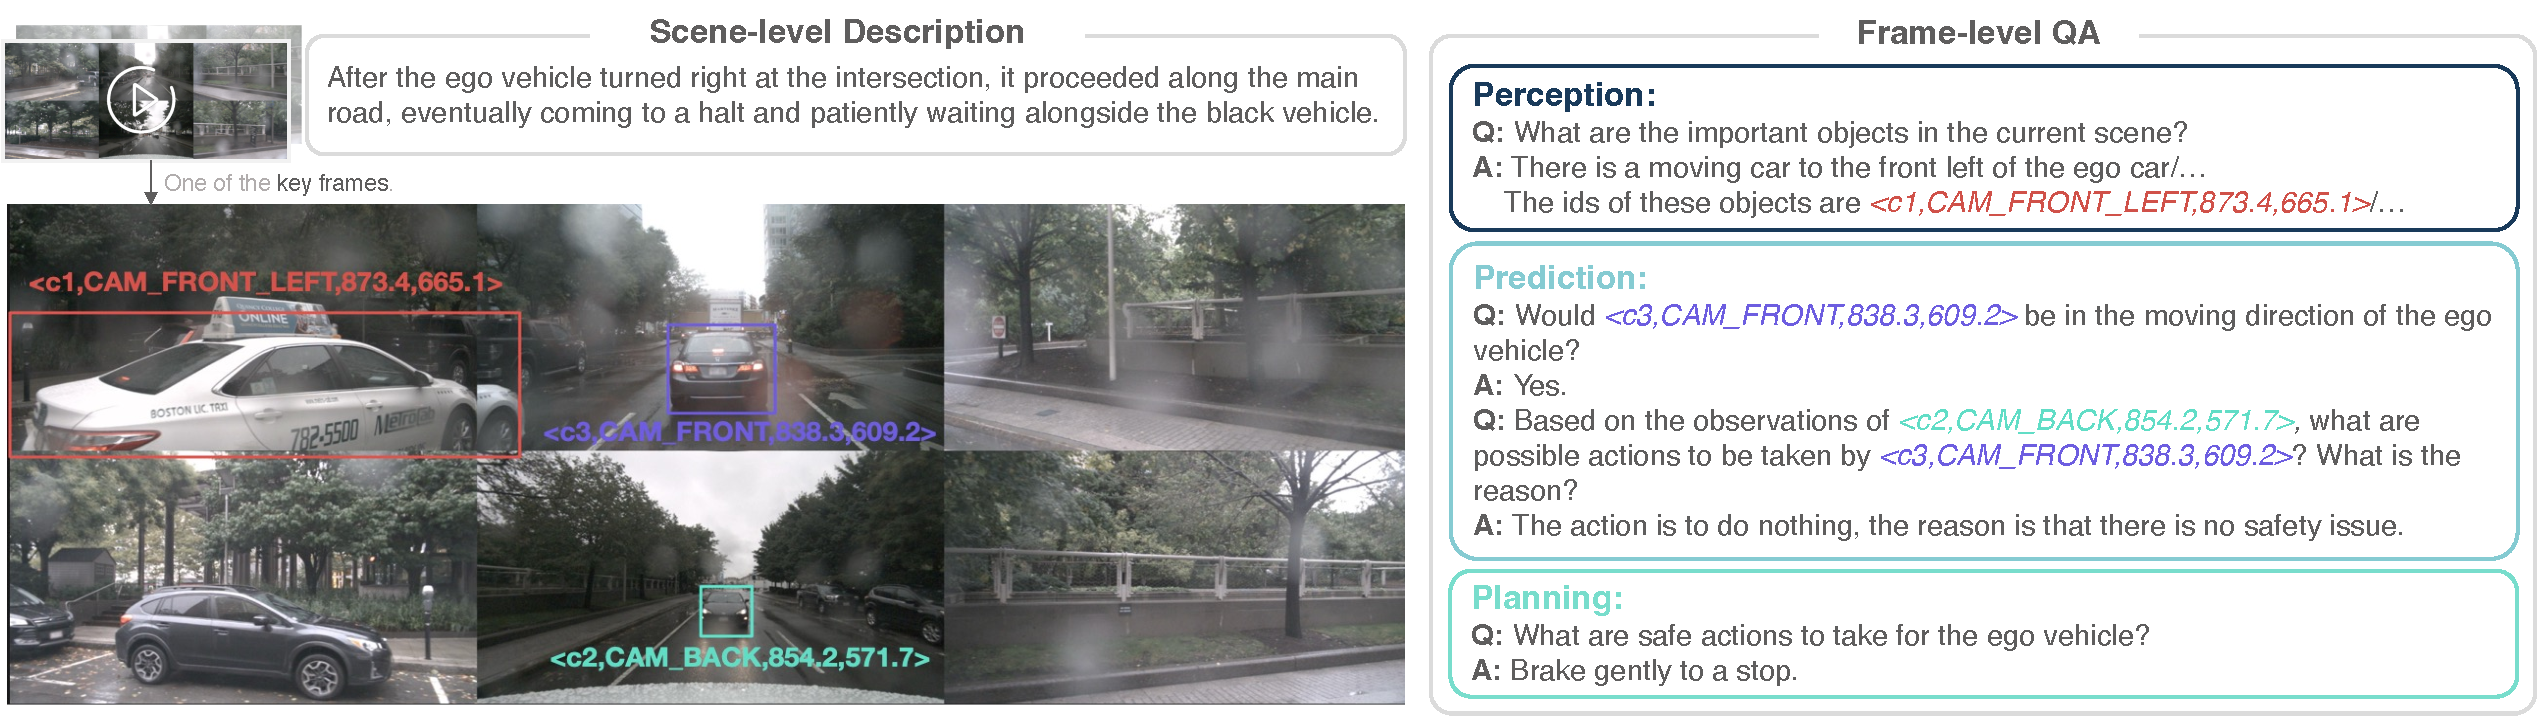
\includegraphics[width=\linewidth]{ch-drivelm/images/nus_data_supp_v2.pdf}
  \caption[Composition of DriveLM-nuScenes]{\textbf{Overall composition of DriveLM-nuScenes.} The dataset comprises scene-level descriptions and frame-level QAs, which divide into three parts: \emph{perception}, \emph{prediction} and \emph{planning}. Objects are encoded as \emph{c tags}, which contain an identifier, the camera, and the centre coordinates of the 2D bounding box of the object in that camera frame.}
  \label{drivelm:fig:composition}
\end{figure}

\subsection{Collection Methodology}\label{drivelm:app:nus_collection}

The labelling is carried out by annotators with driving experience, who are given the stitched images of the six nuScenes cameras. As shown in Fig.~\ref{drivelm:fig:nus_anno_pipeline} (left), the annotation process has three steps: selecting key frames from video clips, choosing key objects within these key frames, and annotating the frame-level QAs of the key frames. Multiple rounds of quality checks then ensure the reliability of the data, and the qualified data are post-processed, as shown in Fig.~\ref{drivelm:fig:nus_anno_pipeline} (right).

\begin{figure}[t]
  \centering
  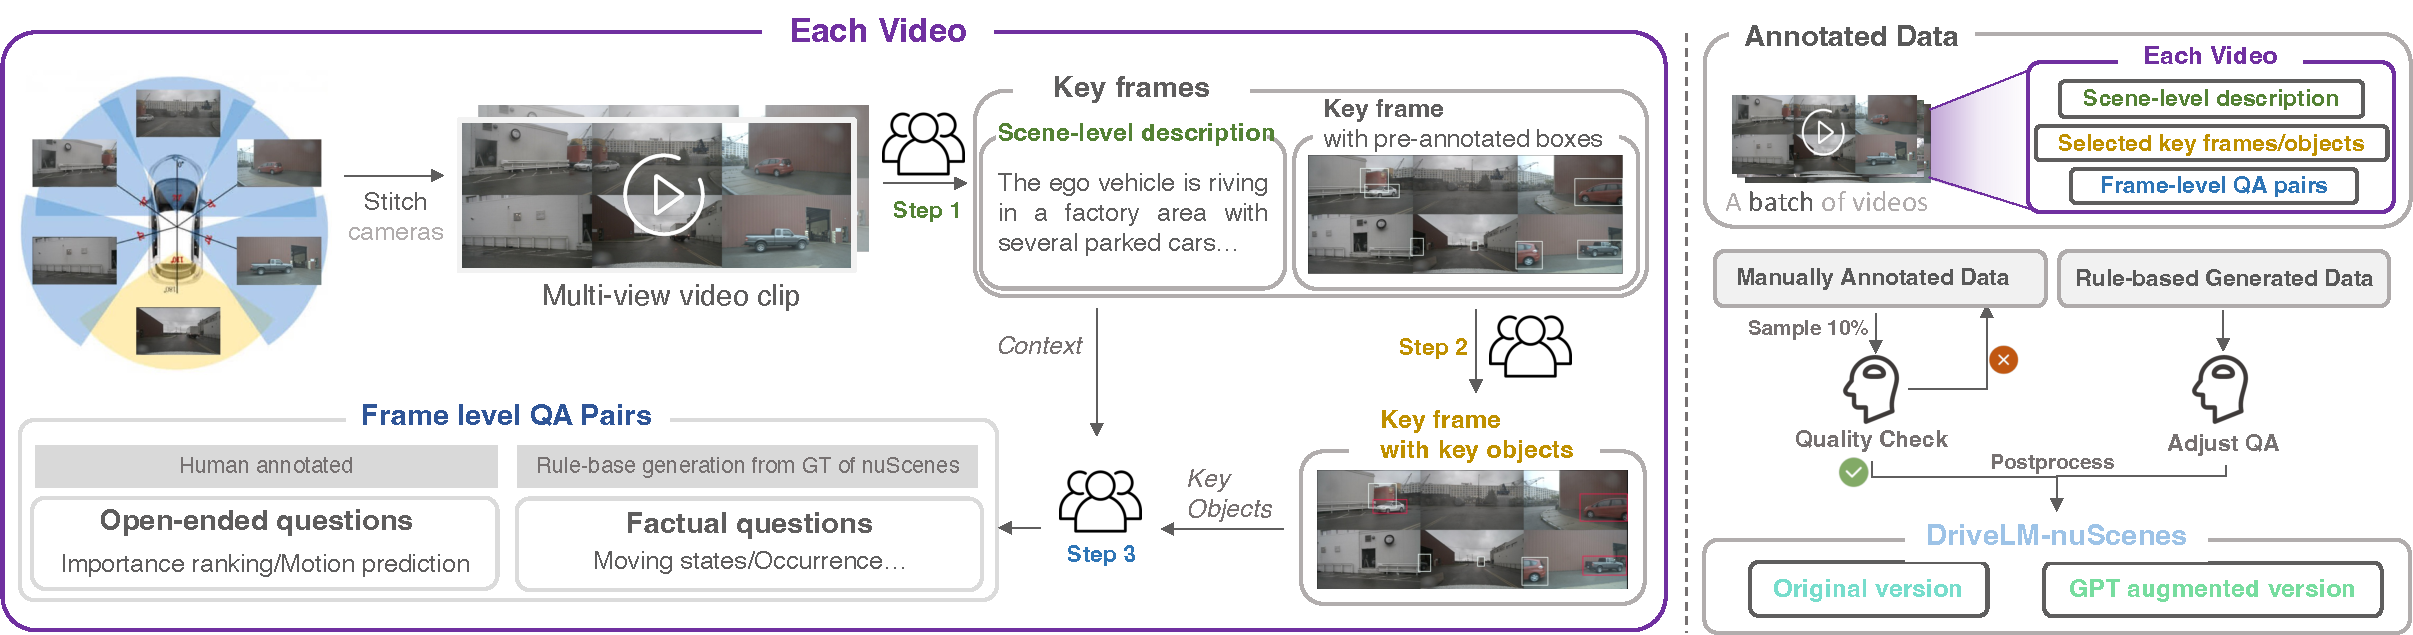
\includegraphics[width=\linewidth]{ch-drivelm/images/nus_pipeline_supp_v2.pdf}
  \caption[Annotation, quality check and post-processing of DriveLM-nuScenes]{\textbf{Left: pipeline of the three-step annotation process.} For each video, the annotators label the key frames, the key objects and the QA attributes step by step. \textbf{Right: quality check and post-processing.} The annotated data are divided into batches, each containing 8 video clips and their annotations. After rigorous quality checks and post-processing, two versions of DriveLM-nuScenes are obtained.}
  \label{drivelm:fig:nus_anno_pipeline}
\end{figure}

\paragraph{Key frame selection.}
Annotators review the entire video clip to pinpoint key frames that are rich in scene information and potentially indicative of future state changes. At the same time, they label the behaviour of the ego vehicle throughout the video clip, which forms the basis of the scene-level description.

\paragraph{Key object selection.}
Annotators identify the objects in the key frames that are relevant to the driving of the ego vehicle, called key objects. To ensure accuracy, pre-annotated bounding boxes based on the ground-truth categories of nuScenes~\cite{caesar2020nuscenes} are provided. Annotators may also designate objects that are not present in the ground truth as key objects if they deem them significant.

\paragraph{QA labelling.}
There are two sets of questions: factual questions and open-ended questions. The answers to factual questions are generated with a rule-based method. The open-ended questions, which are carefully designed in advance, are answered manually by the annotators. Options are provided for most manually annotated questions, together with an ``Other -- Fill in the Blank'' option for flexibility. Free-form questions additionally allow annotators to ask their own questions about the current frame.

\paragraph{Quality check.}
Besides establishing clear criteria and applying automatic checks at each annotation step, we conduct rigorous manual quality checks. The final data are organised into batches, each comprising 8 video clips together with their scene-level descriptions, the key frames and key objects selected from these clips, and the QAs of each key frame. Quality inspectors receive explicit standards on which to base their assessment of data eligibility. For manually annotated data, if the accuracy of the annotations in a batch falls below expectations, we compile feedback on the issues encountered and ask the annotators to re-annotate the entire batch. For data generated from the ground truth, the inspectors manually adjust inconsistent or unreasonable QAs.

\paragraph{Post-processing.}
Because the annotators are Chinese speakers, the labelled data are translated into English. We first establish mappings between Chinese and English with a vocabulary. Texts that cannot be mapped are translated with GPT-3.5, and the GPT outputs are then checked and corrected manually. We also provide a version augmented by GPT-3.5, using the prompt in Table~\ref{drivelm:tab:refine}.

\begin{table}[t]
  \centering
  \caption[Prompt for the GPT-refined version of DriveLM-nuScenes]{\textbf{Prompt for the GPT-refined version of DriveLM-nuScenes.} This pattern was selected from 50 different prompts to perform the refinement.}
  \label{drivelm:tab:refine}
  \begin{tcolorbox}[colback=gray!10, colframe=black, width=\linewidth, arc=1mm, auto outer arc, boxrule=0.5pt, fontupper=\small]
    \raggedright
    \texttt{\textcolor{blue}{Messages} = [}\par\smallskip
    \texttt{\{"role": "system", "content": f"""}You are an English improver.\texttt{"""\},}\par\smallskip
    \texttt{\{"role": "user", "content": f"""}I have a question and answer that I need you to help me modify and embellish, please make a few simple changes to the content in written language and keep the meaning same, you only need to answer the changes to: \texttt{\{\textcolor{blue}{QA}\}"""\}]}
  \end{tcolorbox}
\end{table}

\subsection{Statistics}\label{drivelm:app:nus_stats}

This section analyses the distribution of the QA categories of DriveLM-nuScenes at the task level and at the object level, and lists templates for all QAs at the task level. The results show the richness of the QA categories, which cover various aspects of autonomous driving, and an abundance of logical relationships sufficient to construct graph-structured QAs.

\begin{figure}[t]
  \centering
  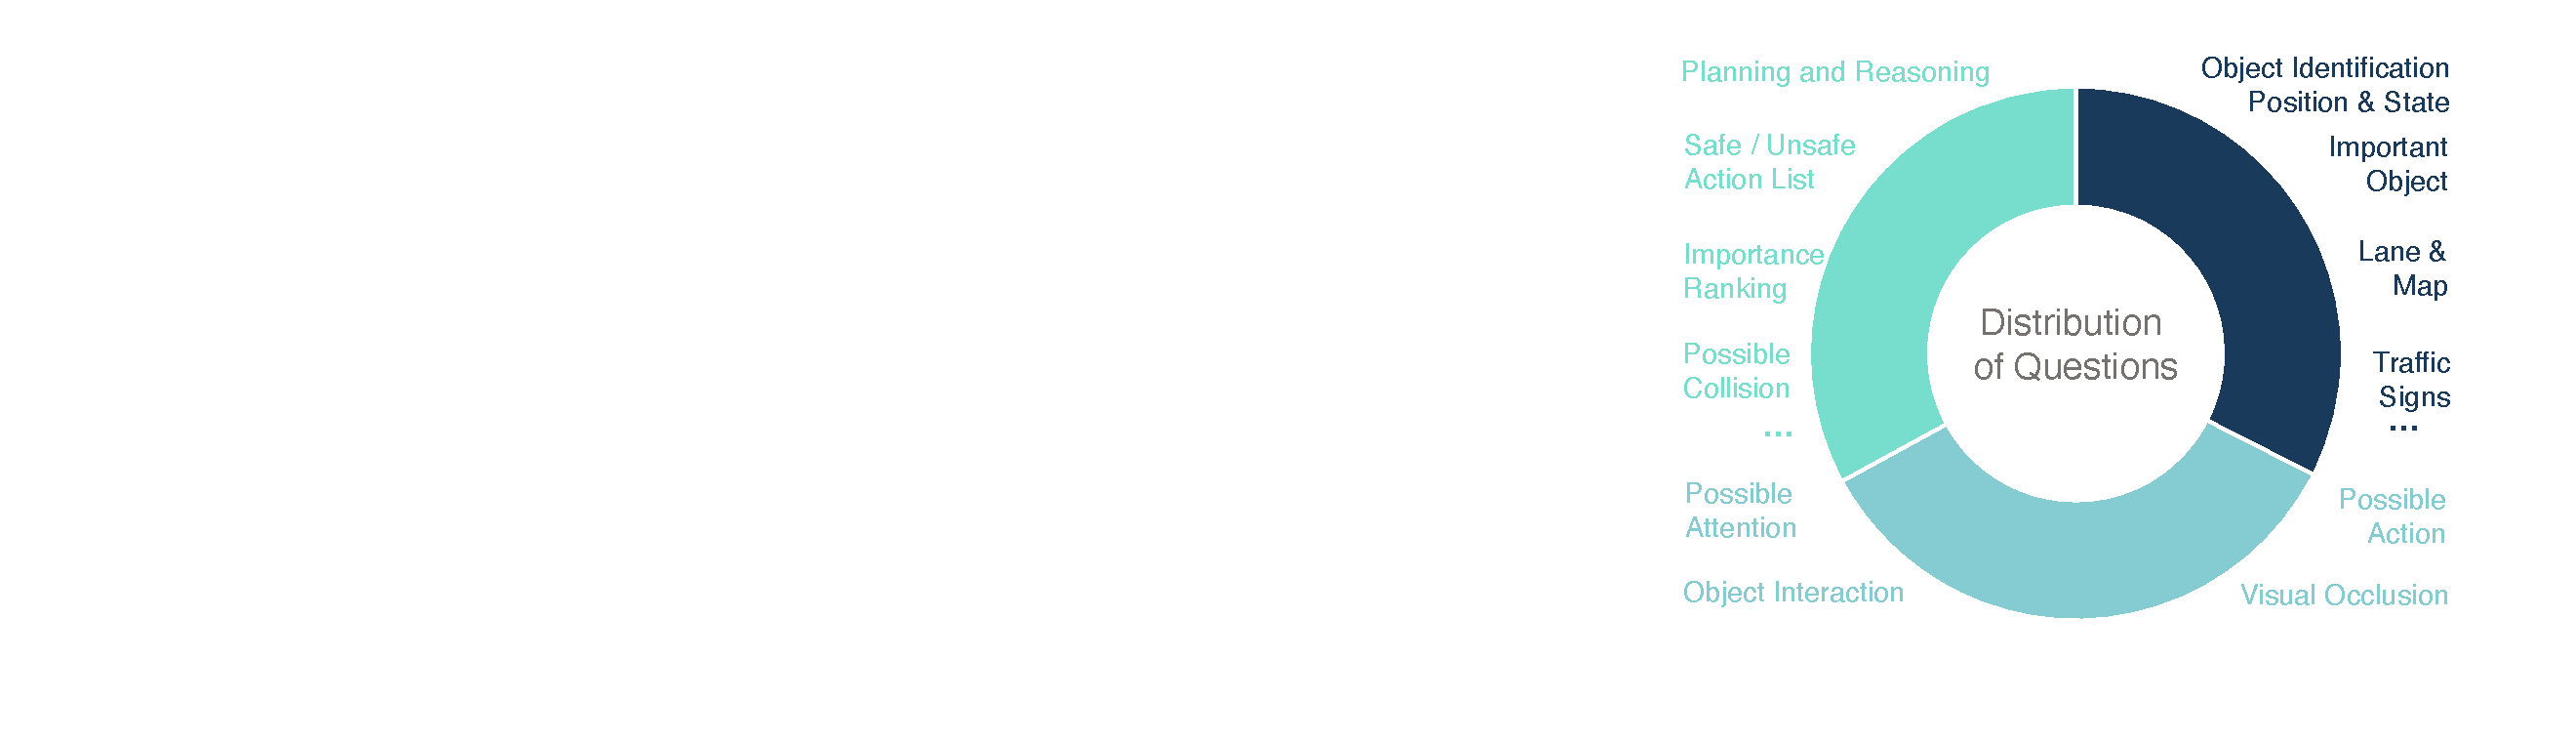
\includegraphics[width=0.6\linewidth]{ch-drivelm/images/data_v8_2_smch.pdf}
  \caption[Question distribution of DriveLM-nuScenes]{\textbf{Question distribution of perception, prediction and planning.} The questions in DriveLM-nuScenes cover various specific aspects of driving and are grouped into perception, prediction and planning. Most of them are annotated by human annotators, which makes the dataset a suitable proxy for human-like driving reasoning.}
  \label{drivelm:fig:data_distribution}
\end{figure}

\begin{figure}[t]
  \centering
  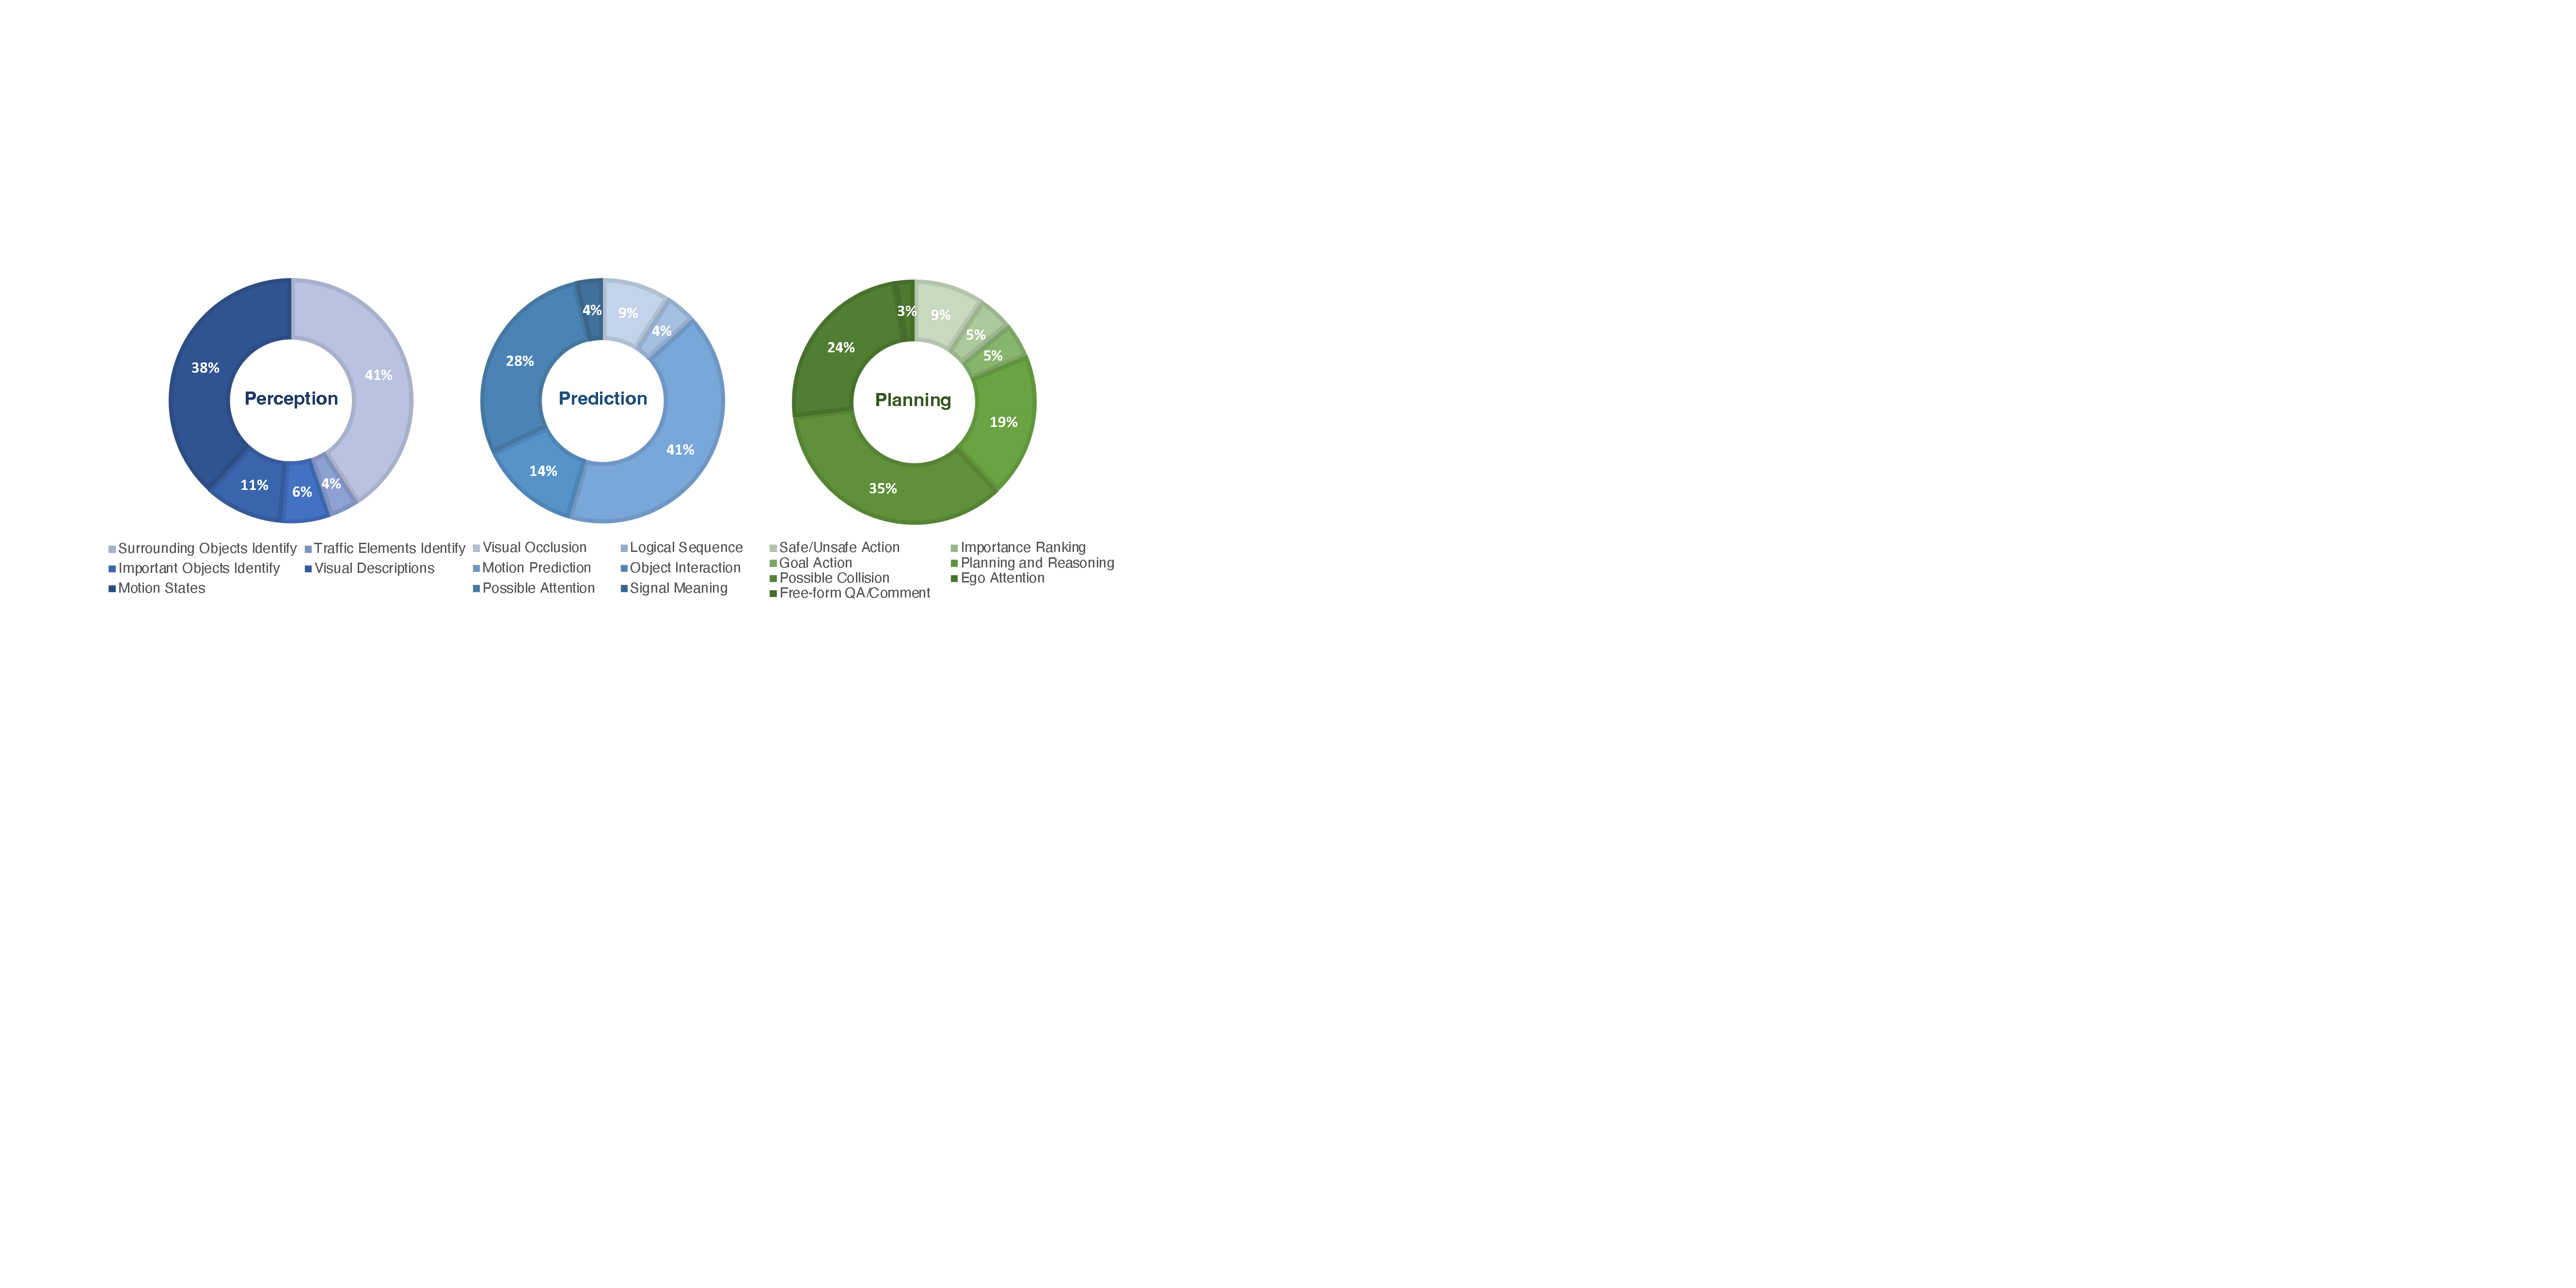
\includegraphics[width=\linewidth]{ch-drivelm/images/nus_stats_supp.pdf}
  \caption[Question types per task in DriveLM-nuScenes]{\textbf{Distribution of question types per task in DriveLM-nuScenes.} Questions are categorised into perception, prediction and planning tasks, each subdivided into more specific question types.}
  \label{drivelm:fig:nus_statis}
\end{figure}

\paragraph{Task level.}
DriveLM-nuScenes forms a benchmark that encompasses various aspects of autonomous driving and connects all stages of human driving logic. Fig.~\ref{drivelm:fig:data_distribution} and Fig.~\ref{drivelm:fig:nus_statis} show the distribution of question types at the task level, and Table~\ref{drivelm:tab:nus_qa} gives example QA templates for all $P_{1-3}$ stages.

\medskip\noindent\begin{minipage}{\linewidth}
  \captionof{table}[Question templates of DriveLM-nuScenes]{\textbf{Question templates of DriveLM-nuScenes at the task level.} The categories correspond to those in Fig.~\ref{drivelm:fig:nus_statis}.}
  \label{drivelm:tab:nus_qa}
\end{minipage}
\nopagebreak
\begin{tcolorbox}[breakable, enhanced, before skip=2pt, colback=gray!10, colframe=black, arc=1mm, boxrule=0.5pt, fontupper=\small\linespread{1.05}\selectfont, parbox=false, before upper={\raggedright\setlength{\parskip}{3pt}}]
\textcolor{blue}{\textbf{Perception}}

\textcolor{blue}{Surrounding Objects Identify}

Q: Please describe the current scene.\\
A: There are two moving cars behind the ego car and two barriers in front of it.

Q: What are objects to the front left/back right/\ldots{} of the ego car?\\
A: There are two barriers to the front left of the ego car.

Q: Are there traffic cones/moving cars/\ldots{} to the front right/back left/\ldots{} of the ego car?\\
A: No.

\textcolor{blue}{Traffic Elements Identify}

Q: Is there any traffic element in the front view?\\
A: Yes, there are some traffic elements in the front view.

Q: Identify all the traffic elements in the front view, categorize them, determine their status, and predict the bounding box around each one. The output should be a list formatted as (c, s, x1, y1, x2, y2), where c represents the category, s denotes the status, and x1, y1, x2, y2 are the offsets of the top-left and bottom-right corners of the box relative to the center point.\\
A: There are three traffic elements in the front view. The information of these traffic elements are [(road sign, go straight, 907.58, 590.67, 992.54, 630.95)\ldots].

\textcolor{blue}{Important Objects Identify}

Q: What are the important objects in the current scene? Those objects will be considered for the future reasoning and driving decision.\\
A: There is a parked truck to the back of the ego car\ldots{} The ids of these objects are <c1,CAM\_BACK,827.5,484.2>\ldots

Q: What is the relative positioning of the important objects in the current scene?\\
A: <c3,CAM\_FRONT,689.2,527.5> is to the front of <c1,CAM\_BACK,827.5,484.2>\ldots

Q: Which lanes are each important object on in the scene?\\
A: <c2,CAM\_FRONT,820.8,473.3> is on the ego lane\ldots

\textcolor{blue}{Visual Description}

Q: What is the visual description of <c2,CAM\_FRONT\_LEFT,415.8,580.8>/\ldots?\\
A: Pedestrian riding a bicycle.

\textcolor{blue}{Motion State}

Q: What is the status of the cars/pedestrians/\ldots{} that are to the front/front right/\ldots{} of the ego car?\\
A: Many cars are parked.

Q: What is the observed status of object <c1,CAM\_FRONT,920.0,509.2>/\ldots?\\
A: Moving.

Q: What is the moving status of object <c1,CAM\_FRONT,920.0,509.2>/\ldots?\\
A: Going ahead.

\textcolor{blue}{\textbf{Prediction}}

\textcolor{blue}{Visual Occlusion}

Q: Which object is most likely to be occluded by <c1,CAM\_FRONT,707.5,472.5>/\ldots? Would this object affect the ego vehicle? Based on this object, what action of the ego vehicle is dangerous?\\
A: The object in front of <c1,CAM\_FRONT,840.8,507.5>, yes, accelerating forward.

\textcolor{blue}{Logical Sequence}

Q: What object should the ego vehicle notice first when the ego vehicle is getting to the next possible location? What is the state of the object that is first noticed by the ego vehicle and what action should the ego vehicle take? What object should the ego vehicle notice second when the ego vehicle is getting to the next possible location? What is the state of the object perceived by the ego vehicle as second and what action should the ego vehicle take? What object should the ego vehicle notice third? What is the state of the object perceived by the ego vehicle as third and what action should the ego vehicle take?\\
A: Firstly notice that <c2,CAM\_FRONT,514.7,462.2>, the state of it is traffic sign, so the ego vehicle should slow down and go ahead. Secondly notice that <c3,CAM\_FRONT,950.3,613.1>, the state of it is traffic sign, so the ego vehicle should slow down and go ahead. Thirdly notice that <c1,CAM\_FRONT,707.5,472.5>, the state of it is going ahead, so the ego vehicle should slow down and go ahead.

\textcolor{blue}{Motion Prediction}

Q: Would <c1,CAM\_FRONT,920.0,509.2>/\ldots{} be in the moving direction of the ego vehicle?\\
A: Yes.

Q: What is the future state of <c1,CAM\_FRONT,920.0,509.2>/\ldots?\\
A: Keep going straight.

Q: Will <c2,CAM\_FRONT,1223.3,598.3>/\ldots{} be in the moving direction of <c1,CAM\_BACK,514.2,503.3>/\ldots?\\
A: No.

\textcolor{blue}{Object Interaction}

Q: Will <c2,CAM\_FRONT,1223.3,598.3>/\ldots{} change its motion state based on <c1,CAM\_BACK,514.2,503.3>/\ldots?\\
A: No.

Q: Based on the observations of <c1,CAM\_BACK,514.2,503.3>/\ldots, what are possible actions to be taken by <c2,CAM\_FRONT,1223.3,598.3>/\ldots? What is the reason?\\
A: The action is to keep going at the same speed, the reason is there is no safety issue.

Q: Based on the observation of <c4,CAM\_FRONT,1071.2,346.2>/\ldots, what actions may <c1,CAM\_FRONT,1126.7,515.0>/\ldots{} take?\\
A: The action is to keep going at the same speed, the reason is there is no safety issue.

\textcolor{blue}{Possible Attention}

Q: In this scenario, what object is most likely to consider <c3,CAM\_FRONT,400.1,717.2>/\ldots?\\
A: The ego vehicle.

Q: Would <c1,CAM\_BACK,514.2,503.3>/\ldots{} take <c3,CAM\_FRONT,400.1,717.2>/\ldots{} into account?\\
A: No.

Q: What object would consider <c1,CAM\_FRONT,985.8,516.7>/\ldots{} to be most relevant to its decision?\\
A: The ego vehicle.

Q: Except for the ego vehicle, what object would consider <c1,CAM\_FRONT,985.8,516.7>/\ldots{} to be most relevant to its decision?\\
A: <c2,CAM\_FRONT,1217.5,511.7>.

\textcolor{blue}{Signal Meaning}

Q: What does <c2,CAM\_BACK\_LEFT,400.8,654.2>/\ldots{} mean?\\
A: No entry.

Q: What kind of traffic sign is <c2,CAM\_BACK\_LEFT,400.8,654.2>/\ldots?\\
A: Traffic cone.

\textcolor{blue}{\textbf{Planning}}

\textcolor{blue}{Safe/Unsafe Action}

Q: In this scenario, what are safe actions to take for the ego vehicle?\\
A: Decelerate gradually without braking, keep going at the same speed.

Q: In this scenario, what are dangerous actions to take for the ego vehicle?\\
A: Accelerate and go ahead, brake suddenly, drive backward, turn right.

\textcolor{blue}{Importance Ranking}

Q: What is the priority of the objects that the ego vehicle should consider? (in descending order)\\
A: <c2,CAM\_FRONT,514.7,462.2>, <c3,CAM\_FRONT,950.3,613.1>, <c1,CAM\_FRONT,707.5,472.5>.

\textcolor{blue}{Goal Action}

Q: What is the target action of the ego vehicle?\\
A: Go straight.

\textcolor{blue}{Planning and Reasoning}

Q: What actions could the ego vehicle take based on <c1,CAM\_FRONT,920.0,509.2>/\ldots? Why take this action and what's the probability?\\
A: The action is to decelerate gradually without braking, the reason is to keep a safe distance, high.

Q: Based on <c3,CAM\_FRONT,1591.1,441.8>/\ldots{} in this scene, what is the most possible action of the ego vehicle?\\
A: Decelerate gradually without braking.

\textcolor{blue}{Possible Collision}

Q: What is the probability of colliding with <c1,CAM\_FRONT,920.0,509.2>/\ldots{} after the ego vehicle goes straight and keeps the same speed/accelerates and goes straight/\ldots?\\
A: Low.

Q: What actions taken by the ego vehicle can lead to a collision with <c1,CAM\_FRONT,920.0,509.2>/\ldots?\\
A: Accelerate and go straight.

\textcolor{blue}{Ego Attention}

Q: What is the traffic signal that the ego vehicle should pay attention to?\\
A: None.

Q: Is <c1,CAM\_FRONT,920.0,509.2>/\ldots{} an object that the ego vehicle should consider in the current scene?\\
A: Yes.

Q: Is it necessary for the ego vehicle to take <c3,CAM\_FRONT,400.1,717.2>/\ldots{} into account?\\
A: Yes.

\textcolor{blue}{Free-form QA/Comment}

Q: What impact does this situation have on driving vehicles?\\
A: The road scene is complex, please slow down.

Q: What's your comment on this scene?\\
A: Pedestrians at the intersection, please be careful and give way.

\ldots
\end{tcolorbox}

\paragraph{Object level.}
Since the QAs in DriveLM-nuScenes revolve around key objects, we also compute statistics at the object level. Fig.~\ref{drivelm:fig:nus_obj_stats} (left) shows the distribution of key object types. Because the questions associated with traffic elements differ substantially from those of the other categories, the statistics of QA types are computed separately for traffic elements and for the remaining categories (Fig.~\ref{drivelm:fig:nus_obj_stats}, right).

\begin{figure}[t]
  \centering
  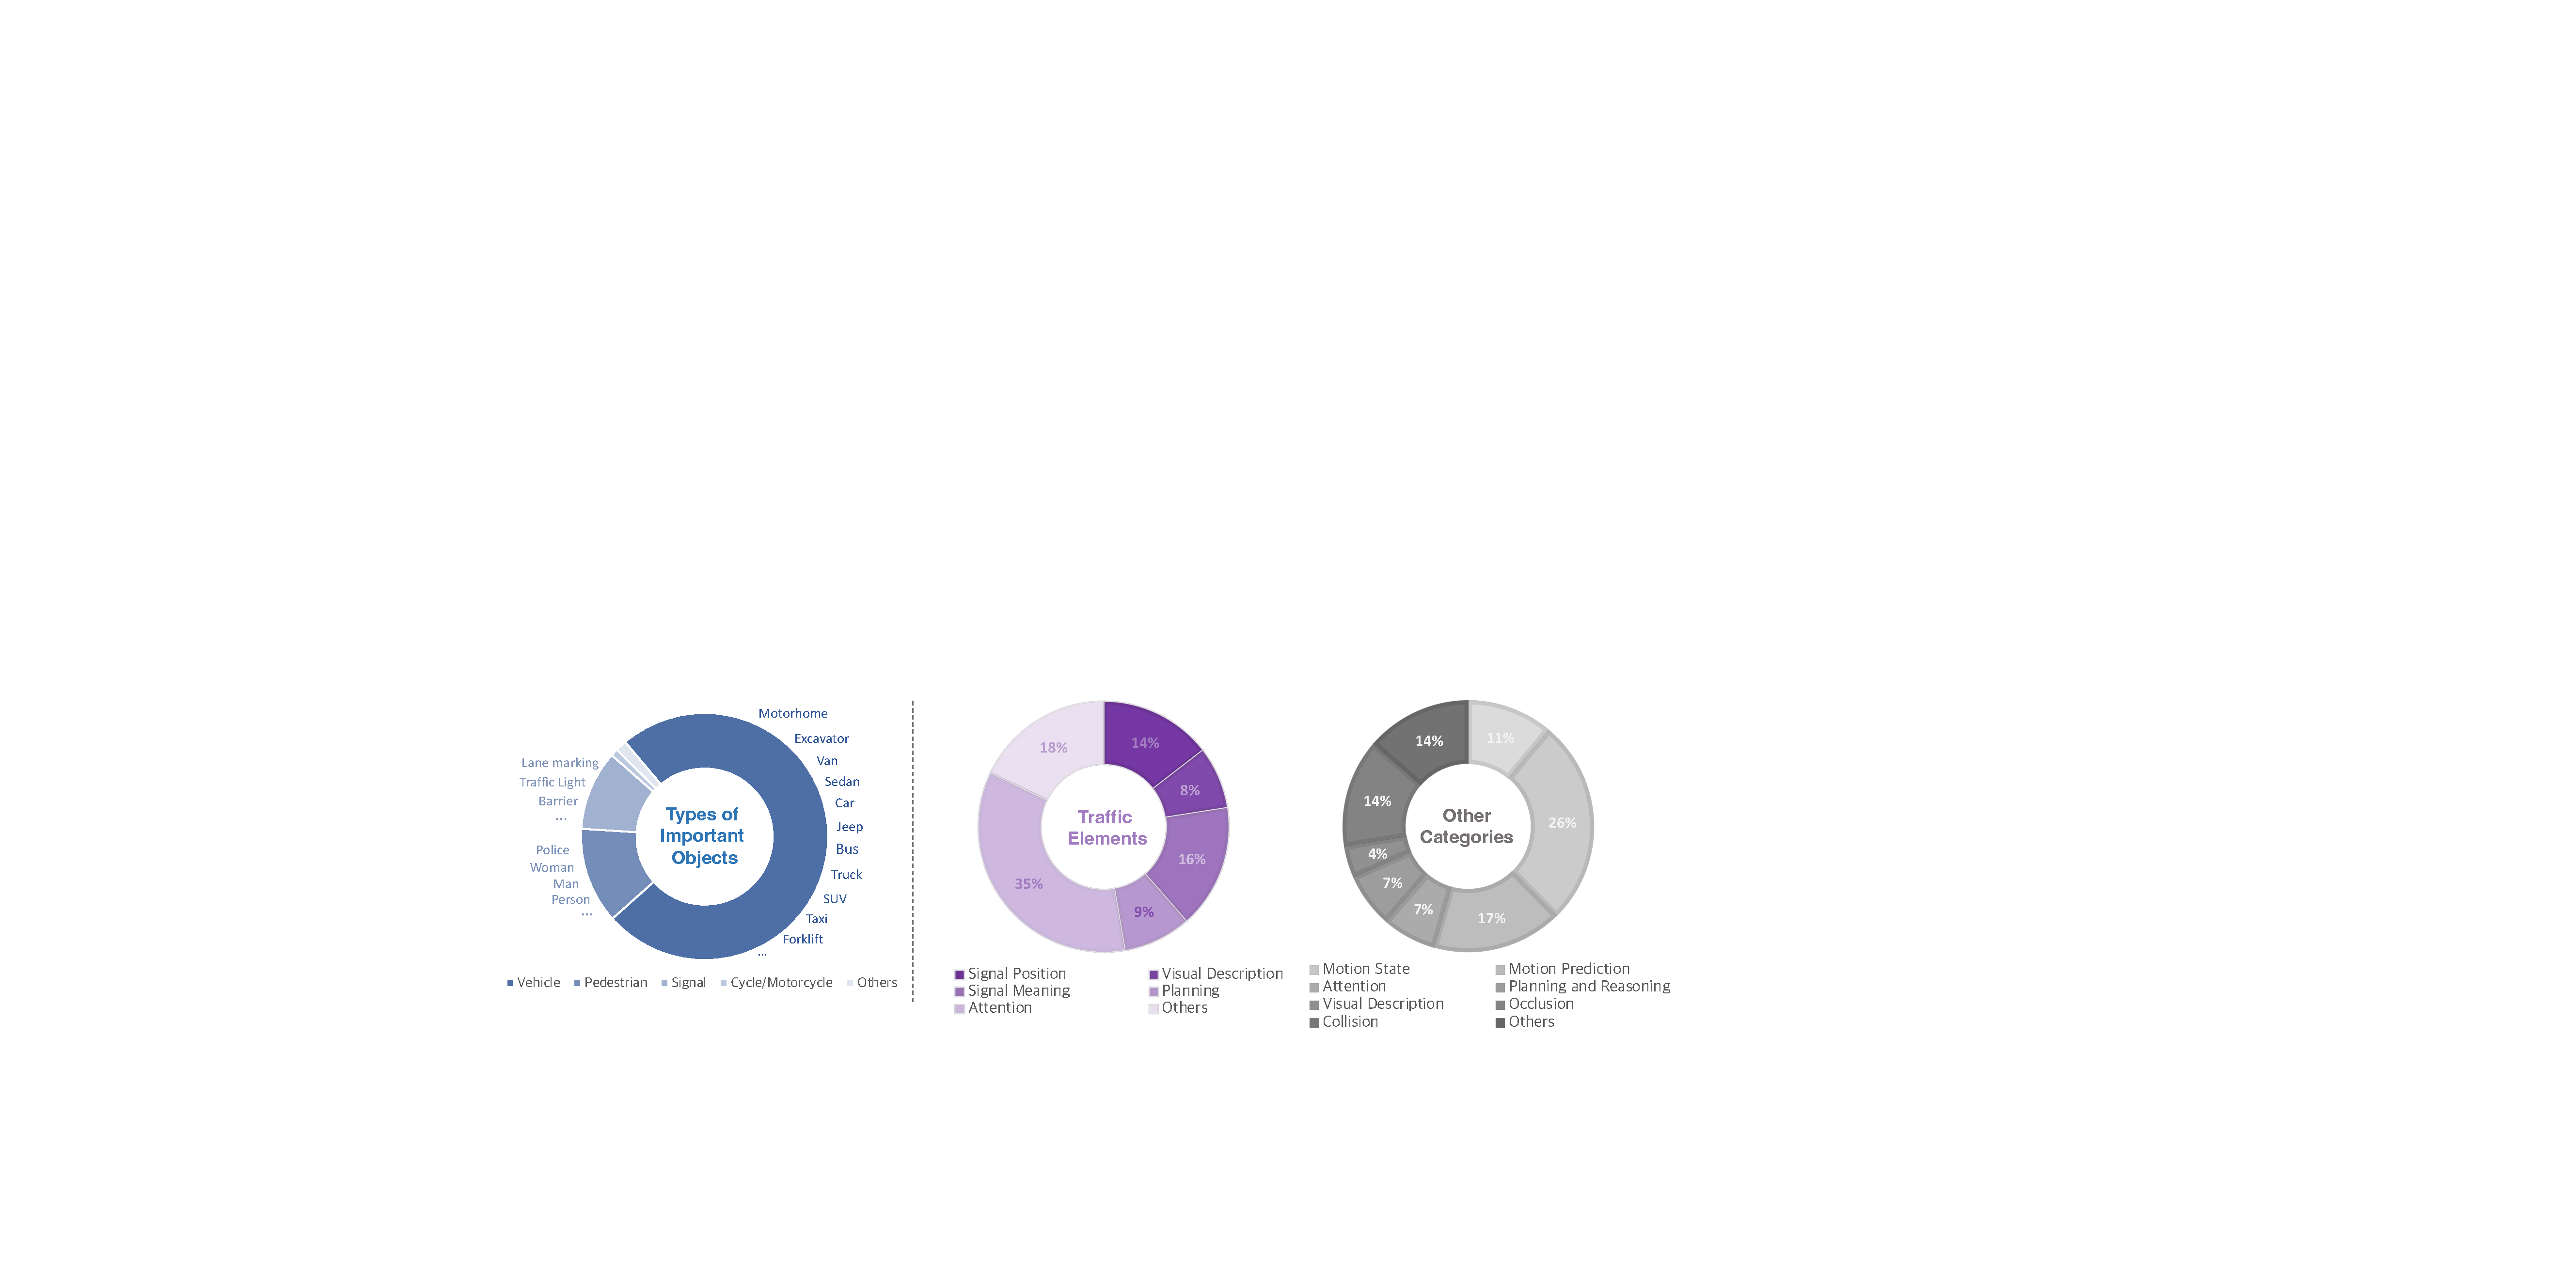
\includegraphics[width=\linewidth]{ch-drivelm/images/nus_objstats_supp.pdf}
  \caption[Key-object statistics of DriveLM-nuScenes]{\textbf{Left: distribution of key objects in DriveLM-nuScenes.} The sub-categories are extracted from the visual descriptions. \textbf{Right: distribution of question types related to different key objects in DriveLM-nuScenes.} Since the questions associated with traffic elements differ substantially from other categories, the statistics of QA types are computed separately for traffic elements and for the remaining categories.}
  \label{drivelm:fig:nus_obj_stats}
\end{figure}

\section{DriveLM-CARLA}\label{drivelm:app:carla}

This section details DriveLM-CARLA: its composition, the PDM-Lite expert and the collection methodology.

\subsection{Dataset Composition}\label{drivelm:app:carla_composition}

DriveLM-CARLA consists of automatically generated frame-level QAs structured as an interconnected graph, shown in Fig.~\ref{drivelm:fig:carla_graph}. In the current version, the dataset consists of questions about the road layout, stop signs, traffic lights and vehicles. Future versions can extend it to more categories such as static objects, weather and traffic signs.

Generating the data in the CARLA simulator allows scalable annotations without any manual effort. The dataset also supports a variety of sensor outputs from CARLA, including semantic segmentation, depth maps and LiDAR, which can be used to train different network architectures. Each question in the graph is designed to facilitate situational reasoning that can be instrumental for answering subsequent questions. As in DriveLM-nuScenes, each question belongs to perception, prediction or planning. For each QA about an object, we save the object ID in addition to the question and answer. This ID is consistent over time, which enables object tracking and temporal reasoning in future studies. The relationships to parent and child questions in the graph are also recorded, allowing efficient traversal of the graph.

\begin{figure}[t]
  \centering
  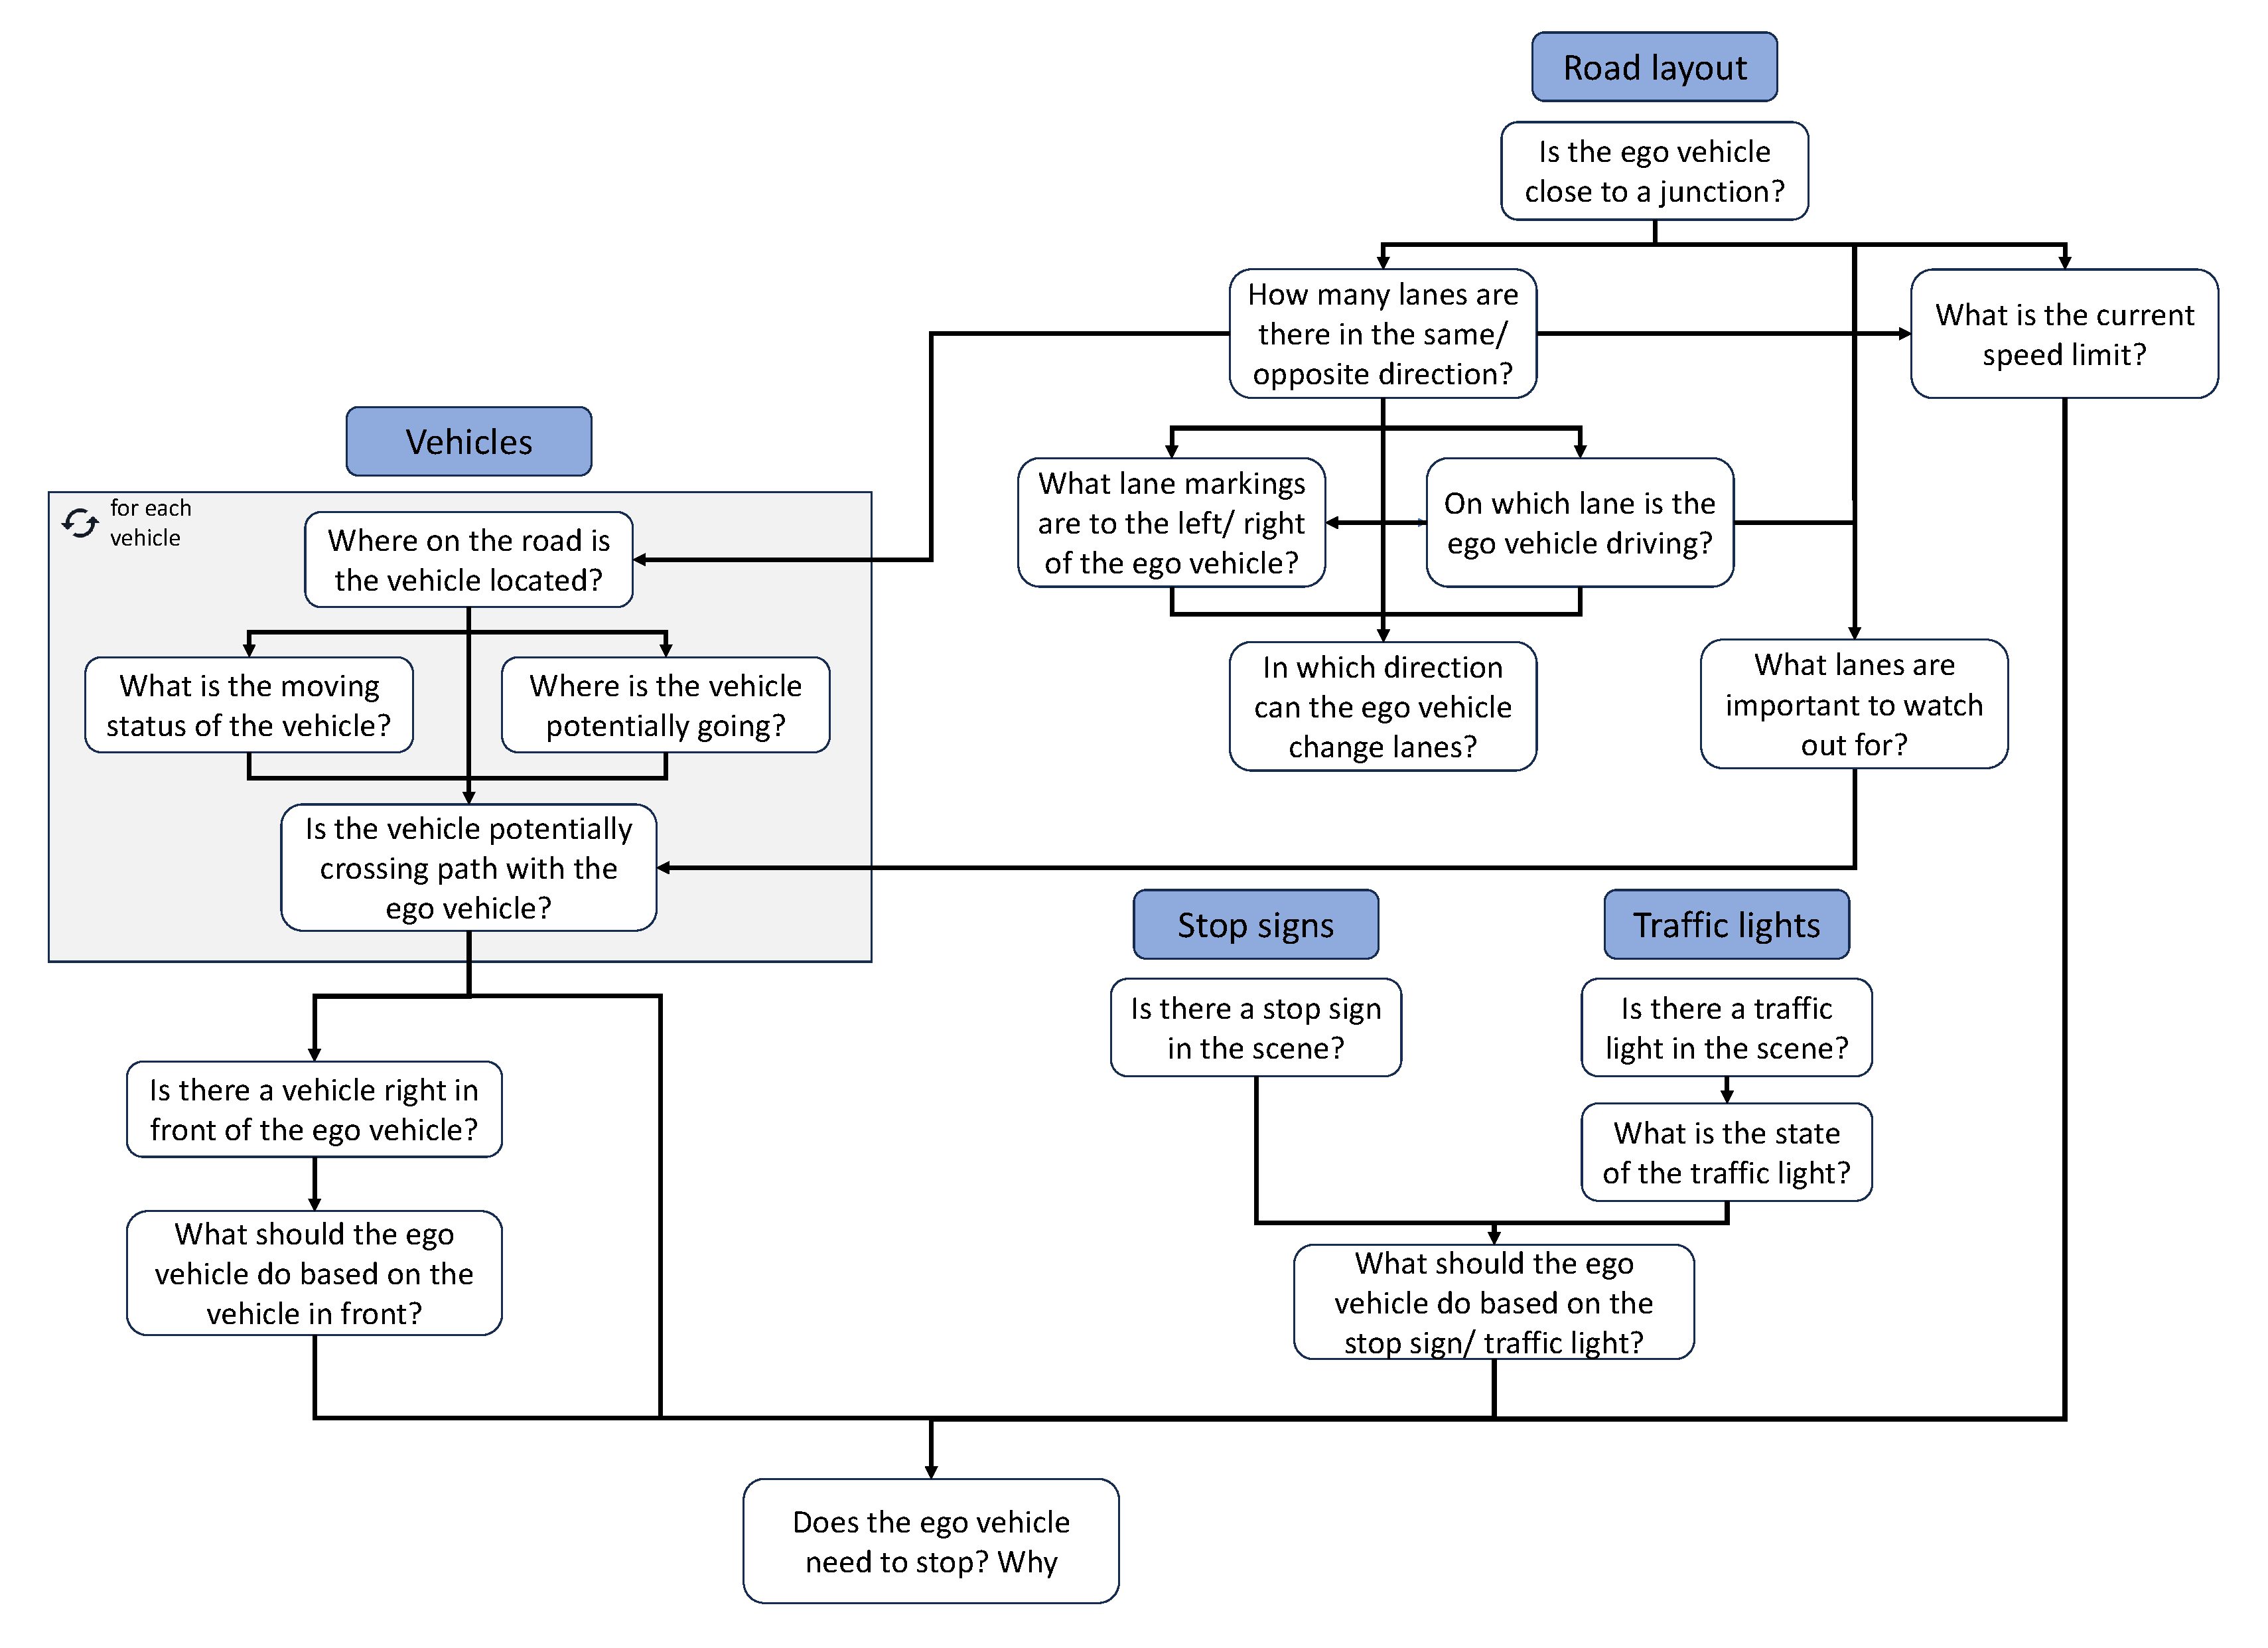
\includegraphics[width=\linewidth]{ch-drivelm/images/carla_graph.pdf}
  \caption[Question graph of DriveLM-CARLA]{\textbf{Detailed flow of the DriveLM-CARLA graph.} The full graph consists of questions and answers about the road layout, traffic lights, stop signs and vehicles.}
  \label{drivelm:fig:carla_graph}
\end{figure}

\subsection{Expert Algorithm: PDM-Lite}\label{drivelm:app:pdm}

Previous CARLA experts, such as the privileged rule-based expert used by TransFuser++~\cite{jaeger2023hidden}, can only solve the scenarios implemented in CARLA Leaderboard 1.0. PDM-Lite~\cite{beisswenger2024pdmlite} is designed to tackle all 38 scenarios of Leaderboard 2.0. It consists of six stages, summarised in Fig.~\ref{drivelm:fig:pdm_lite}.

\begin{figure}[t]
  \centering
  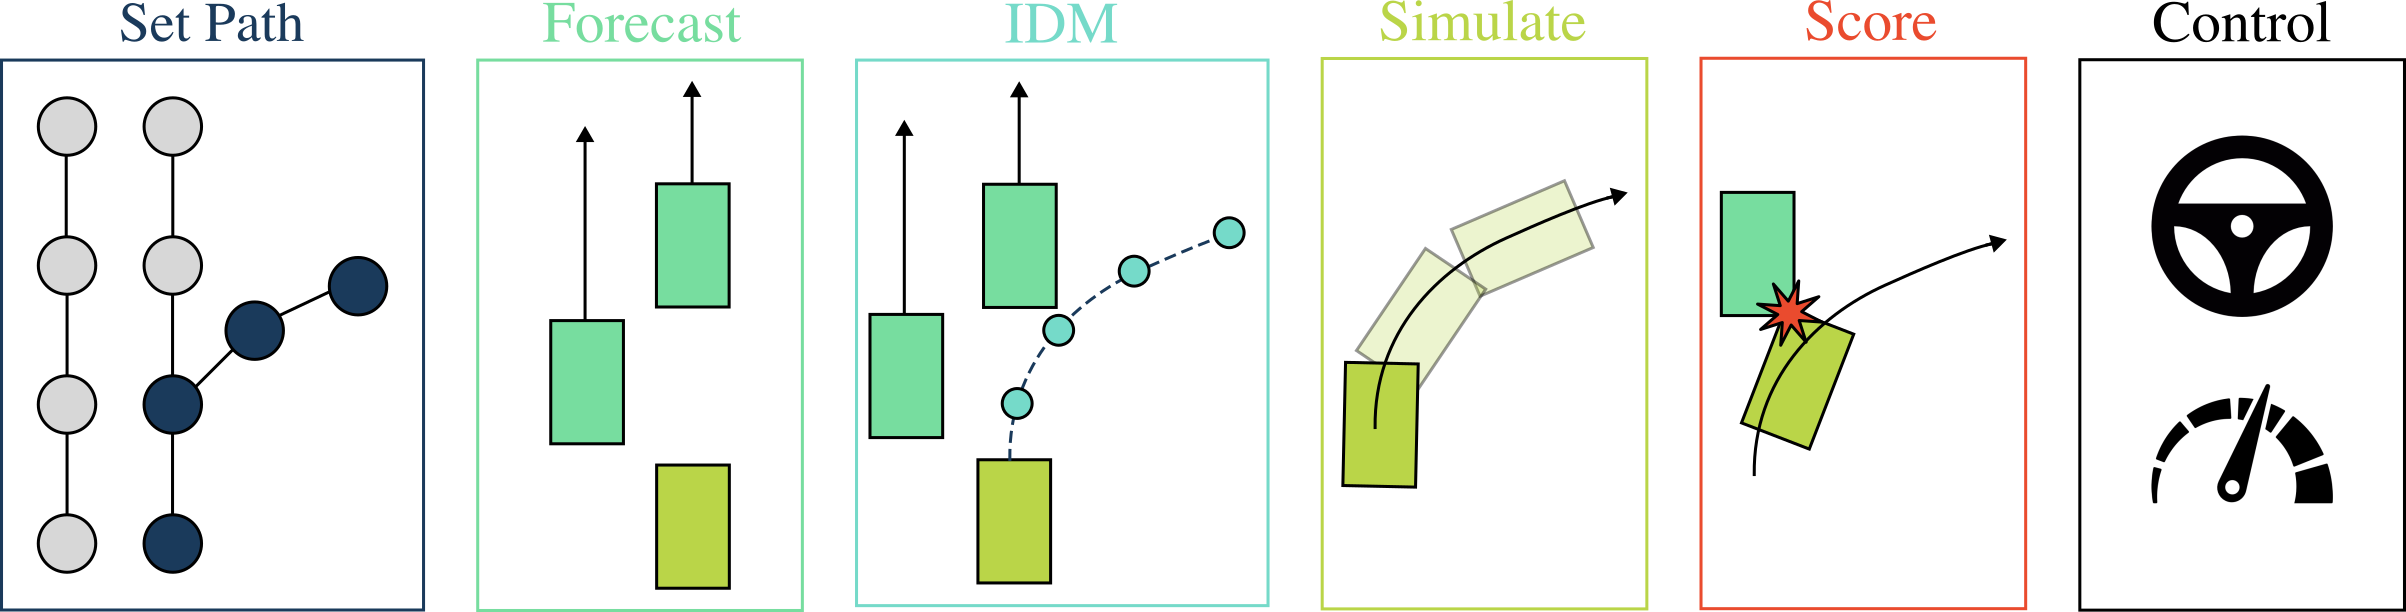
\includegraphics[width=\linewidth]{ch-drivelm/images/PDM-Lite.png}
  \caption[The six stages of PDM-Lite]{\textbf{PDM-Lite.} The new planner, designed to handle all 38 scenarios of CARLA Leaderboard 2.0, has six stages, detailed in Appendix~\ref{drivelm:app:pdm}.}
  \label{drivelm:fig:pdm_lite}
\end{figure}

\paragraph{Path planning.}
\begin{sloppypar}
First, PDM-Lite creates a dense path of spatially equidistant points with an A* planning algorithm, given sparse target points (up to 200\,m apart) from the leaderboard module. The plan is based on the HD map of the town provided by CARLA. Information such as speed limits and distances to the next traffic light or stop sign is added to the different sections of the route to be traversed. To handle scenarios that require leaving the default path, a short segment of the route where the scenario will be spawned is shifted laterally towards an adjacent lane. Examples of such scenarios are \mbox{\emph{Accident}}, \mbox{\emph{ConstructionObstacle}}, \mbox{\emph{ParkedObstacle}}, \mbox{\emph{VehicleOpensDoor}}, \mbox{\emph{AccidentTwoWays}}, \mbox{\emph{ConstructionObstacleTwoWays}}, \mbox{\emph{ParkedObstacleTwoWays}}, \mbox{\emph{VehicleOpensDoorTwoWays}} and \mbox{\emph{YieldToEmergencyVehicle}}.
\end{sloppypar}

\paragraph{Agent forecasting.}
PDM-Lite forecasts the dynamic agents over a horizon of 2\,s with a temporal resolution of 20\,Hz. Since the paths and controls of the other actors are not known in advance, we assume that they maintain their previous controls and apply similar ones in the near future. Using a kinematic bicycle model with parameters taken from~\cite{Chen2021ICCVa}, PDM-Lite forecasts the motion of the other agents under this constant-action assumption, similar to the expert of~\cite{jaeger2023hidden}. Only actors closer than 50\,m to the ego agent are forecast.

\paragraph{IDM target speed.}
A target speed proposal is generated with the Intelligent Driver Model~\cite{treiber2000idm}. While the original IDM selects only one vehicle as the leading actor, we apply it iteratively to all vehicles, pedestrians, non-green traffic lights and stop signs that intersect the path ahead of the ego vehicle. Once the leading actors are selected, a target speed is determined for each of them using the parameters summarised in Table~\ref{drivelm:tab:pdm}. The minimum of these speeds is the final target speed proposal for that time step.

\begin{table}[t]
  \centering
  \caption[IDM parameters of PDM-Lite]{\textbf{Target speed proposal by IDM.} PDM-Lite uses IDM to select a target speed. The parameters for the desired net distance and the desired time headway differ with the type of the leading actor: vehicles, bicycles / stop signs / traffic lights / walkers / static objects (\eg, construction signs).}
  \label{drivelm:tab:pdm}
  \begin{adjustbox}{max width=\textwidth}
  \begin{tabular}{l|l|l}
    \toprule
    \textbf{Parameter} & \textbf{Value} & \textbf{Description} \\
    \midrule
    $v_0$ & $0.72\,v_\textrm{lane}$ & Desired velocity: 72\% of the speed limit \\
    $s_0$ & $4.0$/$2.0$/$6.0$/$4.0$/$2.0$\,m & Desired net distance to the leading agent \\
    $T$ & $0.25$/$0.1$/$0.1$/$0.1$/$0.1$\,s & Desired time headway to the leading agent \\
    $a$ & $24.0\,\textrm{m\,s}^{-2}$ & Maximum acceleration of the ego vehicle \\
    $b_{v \leq 6.02}$ & $8.7\,\textrm{m\,s}^{-2}$ & Maximum deceleration of the ego vehicle if $v \leq 6.02$ \\
    $b_{v > 6.02}$ & $3.72\,\textrm{m\,s}^{-2}$ & Maximum deceleration of the ego vehicle if $v > 6.02$ \\
    $\delta$ & $4.0$ & Acceleration exponent \\
    \bottomrule
  \end{tabular}
  \end{adjustbox}
\end{table}

\paragraph{Simulation.}
The trajectory with the proposed target speed is simulated for 2\,s at 20\,Hz by alternately applying the longitudinal controller (described below) and a kinematic bicycle model. The proposal is thereby converted into an expected sequence of ego-vehicle bounding boxes in closed loop.

\paragraph{Scoring.}
Having forecast the bounding boxes of all actors, we check for intersections between the bounding boxes of the simulated ego vehicle and those of other vehicles, and score the motion of the ego vehicle accordingly: if an intersection with a non-leading and non-rear-end vehicle is detected, the IDM target speed proposal is rejected and the target speed is set to zero.

\paragraph{Controllers.}
Controlling the vehicle requires three values: steering, throttle and brake. The steering value can be estimated directly from the location, velocity and path of the ego vehicle. We use a lateral PID controller for this, similar to~\cite{jaeger2023hidden}, which minimises the angle to a selected point along the path ahead. For throttle and brake, we employ a linear regression model on features extracted from the current speed and the target speed.

\paragraph{Results.}
The performance of PDM-Lite is evaluated on the 20 official validation routes of Leaderboard 2.0. Table~\ref{drivelm:tab:pdm_results} presents the results of evaluations with three different seeds. Routes 0--9 and 10--19 are identical except for the weather conditions, which provides an additional measure of performance variance. Since PDM-Lite uses privileged information, its variance in performance is not due to the different weather parameters but to the random initialisation of the surrounding traffic.

\begin{table}[t]
  \centering
  \caption[PDM-Lite on the official CARLA validation routes]{\textbf{PDM-Lite on the official CARLA validation routes.} Driving performance for each route: Driving Score (DS), Route Completion (RC), Infraction Score (IS), Normalised Driving Score (NDS) and Normalised Infraction Score (NIS), together with the average and the standard deviation over 3 seeds. Routes 0--9 are identical to routes 10--19, except for the weather (which PDM-Lite ignores) and the traffic behaviours.}
  \label{drivelm:tab:pdm_results}
  \small
  \begin{adjustbox}{max width=\textwidth}
  \begin{tabular}{c|c|c|c|c|c}
    \toprule
    \textbf{Route} & \textbf{DS} & \textbf{RC} & \textbf{IS} & \textbf{NDS} & \textbf{NIS} \\
    \midrule
    0 & 14.0 {\color{gray}\footnotesize $\pm 0.0$} & 100.0 {\color{gray}\footnotesize $\pm 0.0$} & 0.14 {\color{gray}\footnotesize $\pm 0.00$} & 48.2 {\color{gray}\footnotesize $\pm 0.0$} & 0.48 {\color{gray}\footnotesize $\pm 0.00$} \\
    1 & 56.2 {\color{gray}\footnotesize $\pm 37.4$} & 71.1 {\color{gray}\footnotesize $\pm 40.9$} & 0.75 {\color{gray}\footnotesize $\pm 0.18$} & 61.9 {\color{gray}\footnotesize $\pm 42.1$} & 0.69 {\color{gray}\footnotesize $\pm 0.32$} \\
    2 & 55.3 {\color{gray}\footnotesize $\pm 14.3$} & 100.0 {\color{gray}\footnotesize $\pm 0.0$} & 0.55 {\color{gray}\footnotesize $\pm 0.14$} & 79.3 {\color{gray}\footnotesize $\pm 6.8$} & 0.79 {\color{gray}\footnotesize $\pm 0.07$} \\
    3 & 18.4 {\color{gray}\footnotesize $\pm 7.8$} & 74.7 {\color{gray}\footnotesize $\pm 35.8$} & 0.34 {\color{gray}\footnotesize $\pm 0.20$} & 38.9 {\color{gray}\footnotesize $\pm 20.4$} & 0.51 {\color{gray}\footnotesize $\pm 0.07$} \\
    4 & 59.8 {\color{gray}\footnotesize $\pm 13.5$} & 100.0 {\color{gray}\footnotesize $\pm 0.0$} & 0.60 {\color{gray}\footnotesize $\pm 0.14$} & 80.5 {\color{gray}\footnotesize $\pm 6.8$} & 0.81 {\color{gray}\footnotesize $\pm 0.07$} \\
    5 & 34.9 {\color{gray}\footnotesize $\pm 9.0$} & 68.0 {\color{gray}\footnotesize $\pm 0.0$} & 0.51 {\color{gray}\footnotesize $\pm 0.13$} & 46.2 {\color{gray}\footnotesize $\pm 5.6$} & 0.68 {\color{gray}\footnotesize $\pm 0.08$} \\
    6 & 36.4 {\color{gray}\footnotesize $\pm 7.9$} & 100.0 {\color{gray}\footnotesize $\pm 0.0$} & 0.36 {\color{gray}\footnotesize $\pm 0.08$} & 70.3 {\color{gray}\footnotesize $\pm 5.1$} & 0.70 {\color{gray}\footnotesize $\pm 0.05$} \\
    7 & 3.5 {\color{gray}\footnotesize $\pm 1.8$} & 100.0 {\color{gray}\footnotesize $\pm 0.0$} & 0.03 {\color{gray}\footnotesize $\pm 0.02$} & 25.7 {\color{gray}\footnotesize $\pm 5.2$} & 0.26 {\color{gray}\footnotesize $\pm 0.05$} \\
    8 & 15.3 {\color{gray}\footnotesize $\pm 3.3$} & 100.0 {\color{gray}\footnotesize $\pm 0.0$} & 0.15 {\color{gray}\footnotesize $\pm 0.03$} & 52.1 {\color{gray}\footnotesize $\pm 3.7$} & 0.52 {\color{gray}\footnotesize $\pm 0.04$} \\
    9 & 73.3 {\color{gray}\footnotesize $\pm 18.9$} & 100.0 {\color{gray}\footnotesize $\pm 0.0$} & 0.73 {\color{gray}\footnotesize $\pm 0.19$} & 89.8 {\color{gray}\footnotesize $\pm 7.2$} & 0.90 {\color{gray}\footnotesize $\pm 0.07$} \\
    \midrule
    10 & 12.8 {\color{gray}\footnotesize $\pm 7.6$} & 100.0 {\color{gray}\footnotesize $\pm 0.0$} & 0.13 {\color{gray}\footnotesize $\pm 0.08$} & 44.0 {\color{gray}\footnotesize $\pm 10.2$} & 0.44 {\color{gray}\footnotesize $\pm 0.10$} \\
    11 & 60.5 {\color{gray}\footnotesize $\pm 32.0$} & 100.0 {\color{gray}\footnotesize $\pm 0.0$} & 0.61 {\color{gray}\footnotesize $\pm 0.32$} & 79.5 {\color{gray}\footnotesize $\pm 18.1$} & 0.79 {\color{gray}\footnotesize $\pm 0.18$} \\
    12 & 52.0 {\color{gray}\footnotesize $\pm 11.3$} & 100.0 {\color{gray}\footnotesize $\pm 0.0$} & 0.52 {\color{gray}\footnotesize $\pm 0.11$} & 78.9 {\color{gray}\footnotesize $\pm 6.5$} & 0.79 {\color{gray}\footnotesize $\pm 0.06$} \\
    13 & 26.3 {\color{gray}\footnotesize $\pm 15.9$} & 49.4 {\color{gray}\footnotesize $\pm 35.8$} & 0.58 {\color{gray}\footnotesize $\pm 0.07$} & 32.2 {\color{gray}\footnotesize $\pm 28.5$} & 0.57 {\color{gray}\footnotesize $\pm 0.11$} \\
    14 & 39.4 {\color{gray}\footnotesize $\pm 20.8$} & 100.0 {\color{gray}\footnotesize $\pm 0.0$} & 0.39 {\color{gray}\footnotesize $\pm 0.21$} & 69.0 {\color{gray}\footnotesize $\pm 11.0$} & 0.69 {\color{gray}\footnotesize $\pm 0.11$} \\
    15 & 24.0 {\color{gray}\footnotesize $\pm 17.2$} & 68.0 {\color{gray}\footnotesize $\pm 0.0$} & 0.35 {\color{gray}\footnotesize $\pm 0.25$} & 35.8 {\color{gray}\footnotesize $\pm 13.8$} & 0.53 {\color{gray}\footnotesize $\pm 0.20$} \\
    16 & 42.0 {\color{gray}\footnotesize $\pm 0.0$} & 100.0 {\color{gray}\footnotesize $\pm 0.0$} & 0.42 {\color{gray}\footnotesize $\pm 0.00$} & 73.9 {\color{gray}\footnotesize $\pm 0.0$} & 0.74 {\color{gray}\footnotesize $\pm 0.00$} \\
    17 & 4.1 {\color{gray}\footnotesize $\pm 1.2$} & 95.3 {\color{gray}\footnotesize $\pm 6.7$} & 0.04 {\color{gray}\footnotesize $\pm 0.01$} & 25.6 {\color{gray}\footnotesize $\pm 5.5$} & 0.27 {\color{gray}\footnotesize $\pm 0.04$} \\
    18 & 12.1 {\color{gray}\footnotesize $\pm 7.9$} & 100.0 {\color{gray}\footnotesize $\pm 0.0$} & 0.12 {\color{gray}\footnotesize $\pm 0.08$} & 43.7 {\color{gray}\footnotesize $\pm 15.6$} & 0.44 {\color{gray}\footnotesize $\pm 0.16$} \\
    19 & 86.7 {\color{gray}\footnotesize $\pm 18.9$} & 100.0 {\color{gray}\footnotesize $\pm 0.0$} & 0.87 {\color{gray}\footnotesize $\pm 0.19$} & 94.9 {\color{gray}\footnotesize $\pm 7.2$} & 0.95 {\color{gray}\footnotesize $\pm 0.07$} \\
    \midrule
    \textbf{Avg.} & \textbf{36.3} {\color{gray}\footnotesize $\pm 28.1$} & \textbf{91.3} {\color{gray}\footnotesize $\pm 21.1$} & \textbf{0.41} {\color{gray}\footnotesize $\pm 0.28$} & \textbf{58.5} {\color{gray}\footnotesize $\pm 25.9$} & \textbf{0.63} {\color{gray}\footnotesize $\pm 0.22$} \\
    \bottomrule
  \end{tabular}
  \end{adjustbox}
\end{table}

\subsection{Collection Methodology}\label{drivelm:app:carla_collection}

\paragraph{Simulator settings.}
We use the CARLA simulator (version 0.9.14) with Leaderboard 2.0~\cite{dosovitskiy2017carla} to generate the dataset. Leaderboard 2.0 introduces two new large maps along with a suite of new scenarios, which increases the diversity of the training and evaluation environments. Town 12 serves as the training town and Town 13 is reserved for evaluation. Each town covers an area of $10\times10$ square kilometres and encompasses varied environments such as rural, residential and urban landscapes that replicate real-world driving conditions. The CARLA team provides a total of 90 training routes, spanning 780.6 kilometres, and 20 evaluation routes, measuring 247.6 kilometres. Every route incorporates multiple driving scenarios. We segment these routes into shorter segments of approximately 150 metres and filter out routes that start and end at the same position. The traffic manager of Leaderboard 2.0 initialises random background traffic around the ego vehicle that consists exclusively of `car' entities. To enrich the dataset, we introduce additional vehicle classes, namely `trucks', `vans', `bicycles' and `motorcycles'. Moreover, we randomise the weather configuration of each training and evaluation route to mimic realistic driving conditions. Night-time settings are excluded because of inadequate illumination in certain regions of the maps: low-light conditions significantly impede the correctness of the automatic labelling, since information about the visibility of objects in the image is hard to obtain.

\paragraph{Data collection.}
We execute the expert on each of the routes and gather a comprehensive set of sensor data: (1) RGB images, (2) LiDAR point clouds, (3) semantic segmentation images, (4) depth maps and (5) bird's-eye-view (BEV) semantic segmentation. While DriveLM-Agent uses only the RGB images, retraining TransFuser++ requires the additional data for its auxiliary tasks. In addition, we extract privileged information from the simulator about the status of the static and dynamic objects in the scene:
\begin{itemize}
  \item \emph{Ego vehicle}: 3D bounding box, speed, brake, id.
  \item \emph{Other vehicles}: 3D bounding box, number of LiDAR points inside the bounding box, distance to the ego vehicle, speed, steering, throttle, brake, id, colour, vehicle type, number of wheels, traffic light state, lane information (\ie, on which road and lane the vehicle is driving), whether the vehicle is in a junction, distance to the next junction, next high-level command.
  \item \emph{Pedestrians}: 3D bounding box, number of LiDAR points inside the bounding box, gender, age, distance to the ego vehicle, speed, id, lane information.
  \item \emph{Traffic lights}: 3D bounding box, distance to the ego vehicle, state, whether it affects the ego vehicle.
  \item \emph{Stop signs}: 3D bounding box, distance to the ego vehicle, whether it affects the ego vehicle.
  \item \emph{Static cars (parked cars)}: 3D bounding box, lane information.
  \item \emph{Landmarks (\eg, speed signs)}: 3D bounding box, distance to the ego vehicle, id, text, value.
  \item \emph{Weather}: weather parameters.
\end{itemize}

\paragraph{Language labels.}
Based on the information extracted from the simulator, we create questions and answers with hand-crafted sentence templates. For more linguistic diversity, and to prevent overfitting to these sentence structures, the sentences could be further augmented with state-of-the-art language models such as GPT-4. In this work, however, we use a version of the dataset that is not augmented.

\section{DriveLM-Metrics}\label{drivelm:app:metrics}

This section details DriveLM-Metrics, which fall into three parts: $P_{1-3}$ VQA metrics, behaviour metrics and motion metrics.

\subsection{\texorpdfstring{$P_{1-3}$}{P1-3} VQA Metrics}\label{drivelm:app:metrics_vqa}

We assess the performance of $P_{1-3}$ with common VQA metrics, and introduce the GPT Score for a more semantically comprehensive evaluation of the QA results. Given the graph structure of the QAs, we also propose the Completeness score for a thorough assessment.

\paragraph{BLEU.}
BLEU~\cite{papineni2002bleu} measures the similarity between a generated text and one or more reference texts by comparing the n-grams of the generated text with those of the references, with higher precision indicating a better match. BLEU is, however, insensitive to semantic nuances and to variations in word order.

\paragraph{ROUGE-L.}
ROUGE-L~\cite{lin2004rouge} computes scores from the longest common subsequence of the model output and the reference answer. Like BLEU, ROUGE assesses the match between generated results and references, the key difference being that ROUGE is based on recall.

\paragraph{METEOR.}
METEOR~\cite{lavie-agarwal-2007-meteor} takes into account precision, recall, stemming, synonymy and word order. It aligns the model output with the references, computes the unigram matches between them, and applies penalties based on chunks, which gives a more nuanced evaluation.

\paragraph{CIDEr.}
CIDEr~\cite{vedantam2015cider} combines elements of BLEU and of vector space models. It treats each sentence as a document, computes its n-gram TF-IDF vector, and uses cosine similarity to measure the semantic consistency between candidate and reference sentences. CIDEr captures matches between n-grams of different lengths and weights the importance of different n-grams through TF-IDF.

\paragraph{SPICE.}
SPICE~\cite{anderson2016spice} first parses the text into a syntactic dependency tree with a probabilistic context-free grammar~\cite{jelinek1992basic}, and then maps the dependency tree to a scene graph with rules. The scene graph describes the objects, attributes and relationships in the text, and the SPICE score is the F-score between the scene graphs of the prediction and of the ground truth.

\paragraph{GPT Score.}
The GPT Score is provided by ChatGPT. Traditional metrics mainly assess performance at the word level and may miss semantic nuances, which can yield unexpected evaluation outcomes. Leveraging the reasoning capabilities of ChatGPT, we use it to gauge the quality of predictions and derive a more rational score. ChatGPT is prompted to assign a numerical score between 0 and 100, with higher scores indicating more accurate predictions. The prompt used for the GPT Score is shown in Table~\ref{drivelm:tab:gpt_score}.

\begin{table}[t]
  \centering
  \caption[Prompt for the GPT Score]{\textbf{Prompt for the GPT Score.} It differs from the prompt used in DriveGPT4~\cite{xu2024drivegpt4}, but the resulting score is similar.}
  \label{drivelm:tab:gpt_score}
  \begin{tcolorbox}[colback=gray!10, colframe=black, width=\linewidth, arc=1mm, auto outer arc, boxrule=0.5pt, fontupper=\small]
    \raggedright
    \texttt{\textcolor{blue}{Messages} = [}\par\smallskip
    \texttt{\{"role": "system", "content": f"""}An evaluator who rates my answer based on the correct answer.\texttt{"""\},}\par\smallskip
    \texttt{\{"role": "user", "content": f"""}Rate my answer based on the correct answer out of 100, with higher scores indicating that the answer is closer to the correct answer, and you should be accurate to single digits like 62, 78, 41, etc. This is the correct answer: \texttt{\{\textcolor{blue}{GT}\}}. This is my answer: \texttt{\{\textcolor{blue}{Pred}\}}.\texttt{"""\}]}
  \end{tcolorbox}
\end{table}

\paragraph{Completeness.}
The Completeness score accounts for how many of the ground-truth questions associated with a frame are answered correctly. For each QA, if the score of the predicted answer is above a threshold, the QA is considered ``correctly answered'' and counts as a correct prediction; otherwise it counts as an incorrect prediction. We then compute the accuracy, \ie, the ratio of the number of correct predictions to the total number of predictions. In our setting, we use the SPICE score with a threshold of 0.5.

\subsection{Behaviour Metrics}\label{drivelm:app:metrics_behavior}

Behaviour predictions are evaluated by classification accuracy, comprising the accuracy of the behaviour and of its speed and steering components. The ground-truth behaviour is derived from the ground-truth future trajectory of the ego vehicle as described in Section~\ref{drivelm:sec:task}: the displacements over each time interval are computed independently for $x$ and $y$ (Eq.~\eqref{drivelm:eq:xy_dist}), their means are mapped to the predefined speed and steering bins, and the two categories together form the behaviour category $(B_{sp},B_{st})$. We compare these categories with the behaviours output by DriveLM-Agent and compute the corresponding accuracies.

\subsection{Motion Metrics}\label{drivelm:app:metrics_motion}

For the motion stage, we use the standard metrics of the nuScenes and Waymo benchmarks: the average and final displacement errors (ADE and FDE) and the collision rate of the predicted trajectory.

\paragraph{ADE.}
The average displacement error is the average L2 distance between the predicted trajectory and the ground-truth trajectory over all predicted horizons. It is the average of the errors at the 1st, 2nd and 3rd second.

\paragraph{FDE.}
The final displacement error is the Euclidean distance between the predicted and the true end point at the last predicted step (the 3rd second).

\paragraph{Collision rate.}
The collision rate is the ratio of the number of test frames in which the predicted trajectory collides with objects to the total number of test frames. The number reported in Table~\ref{drivelm:tab:arch} is the average of the collision rates at the 1st, 2nd and 3rd second.

ADE, FDE and the collision rate are computed with the convention of UniAD~\cite{hu2023uniad}, not that of ST-P3~\cite{hu2022stp3}. For example, for the FDE and the collision rate at the 3rd second, the UniAD convention considers the error or collision rate at this time step only, whereas the ST-P3 convention averages them over 0.5, 1, 1.5, 2, 2.5 and 3 seconds; see the discussion in the UniAD repository\footnote{\raggedright\url{https://github.com/OpenDriveLab/UniAD/commit/ffac1a69a6d01c9dca5cd2ed751007896df351f8}} for details. Moreover, errors reported on the full nuScenes validation set in prior work are not directly comparable with results on the DriveLM-nuScenes validation split, a challenging subset of it that consists only of keyframes with intention changes.

\section{DriveLM-Agent}\label{drivelm:app:agent}

This section details the graph prompting scheme and the trajectory tokenisation of DriveLM-Agent.

\subsection{Prompting with Context}\label{drivelm:app:agent_context}

The content of the context differs between training and inference, following the teacher-forcing setting~\cite{lamb2016professor,toomarian1992learning} generally adopted in recurrent networks. During training, for each edge $e\in E$ of a frame, the child question is appended with the ground-truth parent QA as context. All QAs are used during training, including those without context, and the objective is next-token prediction, the standard approach in language modelling. During inference, the model is applied interactively over multiple rounds to obtain the context predictions required as inputs for each child question. Specifically, the model is prompted with the five stages of questions in the sequential order $P_1$, $P_2$, $P_3$, $B$, $M$. In this order, the model can only answer the questions of a succeeding stage after predicting the answers of the preceding stages.

\subsection{Trajectory Tokenisation}\label{drivelm:app:agent_tokenisation}

To generate action sequences, \ie, future trajectories of the ego vehicle, directly with the language model used for building the graph, we adopt the method of RT-2~\cite{zitkovich2023rt2}, which discretises and tokenises the continuous trajectory.

We first analyse the distribution of the future trajectories in the nuScenes dataset. To convert the continuous $(x,y)$ coordinate space into a discrete set of actions, we partition each coordinate axis into 256 intervals. This granularity ensures sufficient detail while keeping the number of tokens manageable for the language model.

Each bin corresponds to a unique token in the vocabulary of the language model. We extract the token IDs of the numeric tokens in the vocabulary. To preserve the ability to express numerical values, single-digit tokens are omitted from this mapping. From the remaining numeric tokens, a subset of 256 token IDs is selected to represent the trajectory data. In addition, two special tokens mark the start and the end of a trajectory sequence: the start-of-trajectory (SOT) token and the end-of-trajectory (EOT) token. This scheme encodes trajectory information as a sequence of tokens that the language model can process: using the mapped vocabulary, the model predicts a future trajectory as a series of tokens, which are then translated back into the coordinate space (Fig.~\ref{drivelm:fig:simple_pipeline}).

\begin{figure}[t]
  \centering
  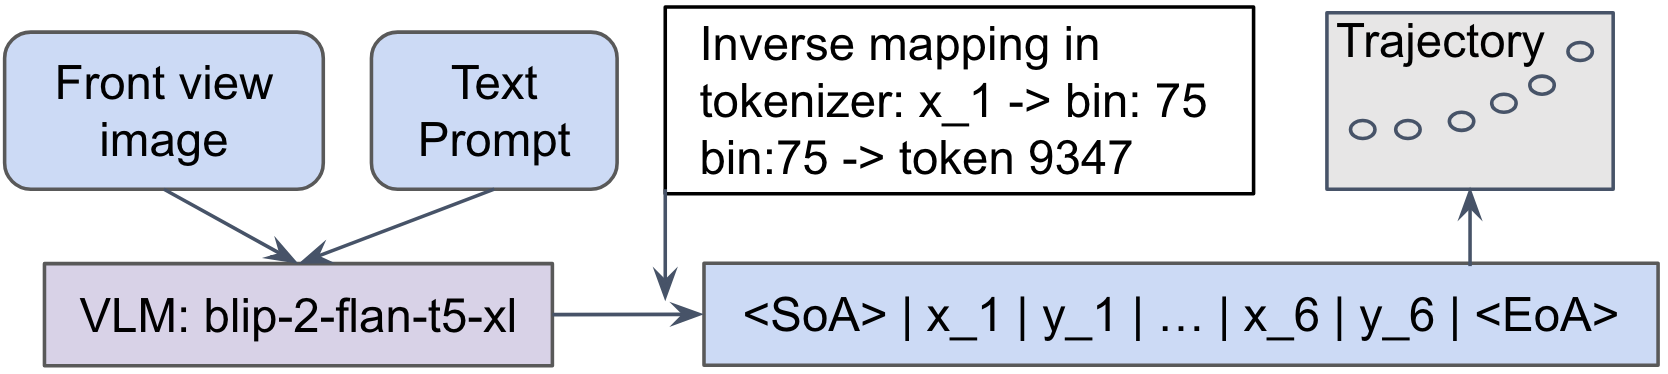
\includegraphics[width=\linewidth]{ch-drivelm/images/rebuttal_simple_pipeline.jpg}
  \caption[Detailed architecture of DriveLM-Agent]{\textbf{Detailed architecture of DriveLM-Agent.} An inverse mapping is designed to embed the real-world trajectory of the ego vehicle into the token space of \texttt{blip-2-flan-t5-xl}.}
  \label{drivelm:fig:simple_pipeline}
\end{figure}

\section{Additional Experimental Details and Results}\label{drivelm:app:exp}

This section gives the implementation details of the experiments in Section~\ref{drivelm:sec:experiments}, additional VQA metrics, a stage-wise ablation, results with another base VLM, and a note on computational complexity.

\subsection{Implementation Details}\label{drivelm:app:impl}

\paragraph{Fine-tuning.}
We set the learning rate to 0.0001, use no learning-rate scheduler, set the random seed to 1234, and otherwise follow the default LoRA~\cite{hu2021lora} configuration. For BLIP-2, we use a maximum sequence length of 400; all other hyperparameters are those of the official BLIP-2 implementation.

\paragraph{Experiments on DriveLM-nuScenes.}
This setting applies to Sections~\ref{drivelm:sec:exp_arch}, \ref{drivelm:sec:exp_question_wise} and~\ref{drivelm:sec:exp_vqa}. During training, all QAs of a frame are used as input, and a subset of them have context (the questions of $P_2$, $P_3$, $B$ and $M$). The contexts are extracted from the ground truth, following the teacher-forcing setting~\cite{lamb2016professor,toomarian1992learning} generally adopted in recurrent networks. At inference, because of the varying complexity of the scenarios, the number of $P_{1-3}$ QAs per frame is highly imbalanced across the dataset, with a variance of over 260 on DriveLM-nuScenes. To balance its impact, we compute the GVQA scores on only a subset of the QAs associated with each frame. To extract this subset, we design a set of QA patterns for each stage based on the questions generally associated with that stage, and ensure that every validation frame has at least one question matching the pattern in each stage. Except for the questions of stage $P_1$, all questions receive context from the QAs of the previous stage, whose answers are derived from the predictions of the preceding steps. Fig.~\ref{drivelm:fig:nus_detailed_results} and Fig.~\ref{drivelm:fig:nus_results} show two examples of the resulting graph structure.

\paragraph{Experiment on Waymo.}
This setting applies to Section~\ref{drivelm:sec:exp_waymo}. The model is trained with the same scheme as above on the \texttt{train} split of DriveLM-nuScenes. Since Waymo has no annotations (not even questions), the questions at inference are devised with rules. Specifically, we reuse the general-purpose perception questions of DriveLM-nuScenes as the starting questions for Waymo. We then check whether the answers mention objects that also occur in the DriveLM-nuScenes annotations, such as ``pedestrians'', ``cars'' or ``trucks'', and automatically generate questions about these matched objects, which serve as the subsequent questions of the prediction and planning stages. Fig.~\ref{drivelm:fig:waymo_results} shows an example of the resulting graph structure.

\paragraph{Experiment on DriveLM-CARLA-ped.}
For the generalisation experiment of Section~\ref{drivelm:sec:exp_carla}, two new questions are added to the graph: (1) \emph{Is there a person in the scene?} and (2), if the answer to the first question is yes, \emph{What should the vehicle do based on the pedestrian that is crossing the road?}, or otherwise \emph{What should the ego vehicle do?}. The answer to the second question is concatenated to the context of the final behaviour question. Fig.~\ref{drivelm:fig:carla_resultsPed} shows three examples.

\subsection{Results with More VQA Metrics}\label{drivelm:app:vqa_metrics}

Table~\ref{drivelm:tab:vqa_more_metrics} reports the setting of Table~\ref{drivelm:tab:vqa} under BLEU-4~\cite{papineni2002bleu}, METEOR~\cite{lavie-agarwal-2007-meteor}, CIDEr~\cite{vedantam2015cider}, ROUGE-L~\cite{lin2004rouge} and the Completeness score. A key observation is that different metrics reflect different trends, and the improvement is not consistent across all of them. This motivates the use of the GPT Score as the main metric for VQA evaluation.

\begin{table}[t]
  \centering
  \caption[More VQA metrics on DriveLM-nuScenes]{\textbf{Graph-structured reasoning facilitates VQA with VLMs} (DriveLM-nuScenes). Completeness (Comp.) measures how many questions of a frame are answered correctly. The improvement trends are not consistent across the conventional metrics, so the GPT Score, which evaluates the performance more comprehensively, is used as the main metric.}
  \label{drivelm:tab:vqa_more_metrics}
  \begin{adjustbox}{max width=\textwidth}
  \begin{tabular}{ll|ccccccc}
    \toprule
    \textbf{Model} & \textbf{Context} & BLEU-4\,$\uparrow$ & METEOR\,$\uparrow$ & CIDEr\,$\uparrow$ & ROUGE-L\,$\uparrow$ & SPICE\,$\uparrow$ & GPT\,$\uparrow$ & Comp.\,$\uparrow$ \\
    \midrule
    \multirow{3}{*}{Off-the-shelf BLIP-2} & None & 0.022 & 3.317 & 0.1185 & 7.205 & 4.336 & 42.97 & 1.064 \\
    & Graph & 0.022 & 3.882 & 0.0771 & 7.397 & 7.710 & 45.21 & 0.859 \\
    & \textit{GT} & \textit{0.022} & \textit{4.397} & \textit{0.0758} & \textit{8.033} & \textit{8.192} & \textit{41.10} & \textit{1.315} \\
    \midrule
    \multirow{3}{*}{DriveLM-Agent} & None & 51.89 & 35.81 & 2.463 & 66.79 & 42.56 & 71.39 & 30.04 \\
    & Graph & 53.09 & 36.19 & 2.786 & 65.58 & 49.54 & 72.51 & 31.66 \\
    & \textit{GT} & \textit{53.06} & \textit{36.64} & \textit{3.069} & \textit{66.69} & \textit{50.29} & \textit{72.94} & \textit{32.41} \\
    \bottomrule
  \end{tabular}
  \end{adjustbox}
\end{table}

\subsection{Stage-wise Context Ablation on Waymo}\label{drivelm:app:waymo_ablation}

Table~\ref{drivelm:tab:waymo_supp} extends the zero-shot generalisation experiment of Table~\ref{drivelm:tab:arch} with more context settings. A key observation is that the higher the accuracy of the behaviour task, the better the performance of the motion task. With more context for the behaviour task, the accuracy improvement comes mainly from the speed accuracy, which in turn affects the FDE.

\begin{table}[t]
  \centering
  \caption[Stage-wise ablation on zero-shot generalisation to Waymo]{\textbf{Zero-shot generalisation across sensor configurations.} $B^{*}$ denotes using the ground-truth behaviour QA as context for the motion task. Results on 1k randomly sampled frames of the Waymo \texttt{val} set after training on DriveLM-nuScenes. The key observation is that the higher the accuracy of the behaviour task, the better the performance of the motion task.}
  \label{drivelm:tab:waymo_supp}
  \begin{adjustbox}{max width=\textwidth}
  \begin{tabular}{l|cc|ccc|cc}
    \toprule
    \multirow{2}{*}{\textbf{Method}} & \textbf{Behaviour} & \textbf{Motion} & \multicolumn{3}{c|}{\textbf{Behaviour ($B$)}} & \multicolumn{2}{c}{\textbf{Motion ($M$)}} \\
    & \textbf{Context} & \textbf{Context} & Acc.\,$\uparrow$ & Speed\,$\uparrow$ & Steer\,$\uparrow$ & ADE\,$\downarrow$ & FDE\,$\downarrow$ \\
    \midrule
    Command Mean & - & - & - & - & - & 7.98 & 11.41 \\
    UniAD-Single & - & - & - & - & - & 4.16 & 9.31 \\
    BLIP-RT-2 & - & - & - & - & - & 2.78 & 6.47 \\
    \midrule
    & None & $B$ & 35.70 & 43.90 & 65.20 & 2.76 & 6.59 \\
    & $P_1$ & $B$ & 38.20 & 43.67 & 70.74 & 2.67 & 6.41 \\
    DriveLM-Agent & $P_2$ & $B$ & 39.52 & 44.20 & \textbf{78.67} & \textbf{2.62} & 6.19 \\
    & $P_3$ & $B$ & 34.62 & 41.28 & 64.55 & 2.85 & 6.89 \\
    & $P_{1-3}$ & $B$ & \textbf{39.73} & \textbf{54.29} & 70.35 & 2.63 & \textbf{6.17} \\
    \midrule
    \textit{BLIP-RT-2} & \textit{-} & $B^{*}$ & \textit{100.0} & \textit{100.0} & \textit{100.0} & \textit{2.41} & \textit{5.79} \\
    \bottomrule
  \end{tabular}
  \end{adjustbox}
\end{table}

\subsection{More VLMs on DriveLM-nuScenes}\label{drivelm:app:more_vlms}

To validate the generality of DriveLM-Agent and to explore whether video input helps in this task, we select LLaMA-Adapter V2 (7B)~\cite{gao2023llamaadapterv2}, which is compatible with both single-frame and multi-frame inputs. The results in Table~\ref{drivelm:tab:llama}, obtained within 9 training epochs, show a performance similar to that of BLIP-2.

Because of the large variety of question types in DriveLM-nuScenes, analysing each question individually would be prohibitively expensive. Instead, we provide a stage-wise ablation of the $P_{1-3}$ context in Table~\ref{drivelm:tab:waymo_supp} and the representative question-wise analysis in Table~\ref{drivelm:tab:question_wise}. Improving the $P_{1-3}$ QA performance under the current question setting is non-trivial, and we found that it had little effect on the final task performance (behaviour and motion). This suggests that the question setup deserves more exploration: with well-chosen questions, the model could be ``prompted correctly'' to understand the scene and perform the downstream task better.

\begin{table}[t]
  \centering
  \caption[Other base VLMs on DriveLM-nuScenes]{\textbf{More VLMs evaluated on DriveLM-nuScenes.} With LLaMA-Adapter V2 as the base model, multi-frame input ($^{*}$) gives a slight improvement.}
  \label{drivelm:tab:llama}
  \begin{adjustbox}{max width=\textwidth}
  \begin{tabular}{l|cc|ccc|cc}
    \toprule
    \multirow{2}{*}{\textbf{Base VLM}} & \textbf{Behaviour} & \textbf{Motion} & \multicolumn{3}{c|}{\textbf{Behaviour ($B$)}} & \multicolumn{2}{c}{\textbf{Motion ($M$)}} \\
    & \textbf{Context} & \textbf{Context} & Acc.\,$\uparrow$ & Speed\,$\uparrow$ & Steer\,$\uparrow$ & ADE\,$\downarrow$ & Col.\,$\downarrow$ \\
    \midrule
    \texttt{blip-2-flan-t5-xl} & Graph & $B$ & 57.49 & \textbf{69.89} & 80.63 & \textbf{1.74} & 1.89 \\
    \rowcolor[gray]{0.9} LLaMA-Adapter V2 & Graph & $B$ & 55.31 & 61.97 & 81.43 & 1.86 & 2.03 \\
    \rowcolor[gray]{0.9} LLaMA-Adapter V2$^{*}$ & Graph & $B$ & \textbf{57.83} & 67.21 & \textbf{83.49} & 1.75 & \textbf{1.69} \\
    \bottomrule
  \end{tabular}
  \end{adjustbox}
\end{table}

\subsection{Computational Complexity}\label{drivelm:app:complexity}

Table~\ref{drivelm:tab:latency} compares the computational complexity of DriveLM-Agent with that of UniAD-Single. A future direction is to cache the vision tokens and to batch the different question patterns, which could fundamentally speed up inference.

\section{Qualitative Results}\label{drivelm:app:qualitative}

This section shows qualitative results of VQA on DriveLM-nuScenes, of generalisation across sensor configurations on Waymo, and of generalisation to unseen objects on DriveLM-CARLA.

\subsection{DriveLM-nuScenes}\label{drivelm:app:qual_nus}

Fig.~\ref{drivelm:fig:nus_detailed_results} shows a detailed example of the GVQA reasoning process on DriveLM-nuScenes, covering the $P_{1-3}$ QAs and the behaviour task. It compares the predicted answers with the ground truth and gives their SPICE and GPT scores. The second question of the prediction stage represents a typical error: with single-frame input, the model often struggles to determine the correct movement status of objects, a judgement that is challenging even for humans. Fig.~\ref{drivelm:fig:nus_results} presents further qualitative results.

\begin{figure}[t]
  \centering
  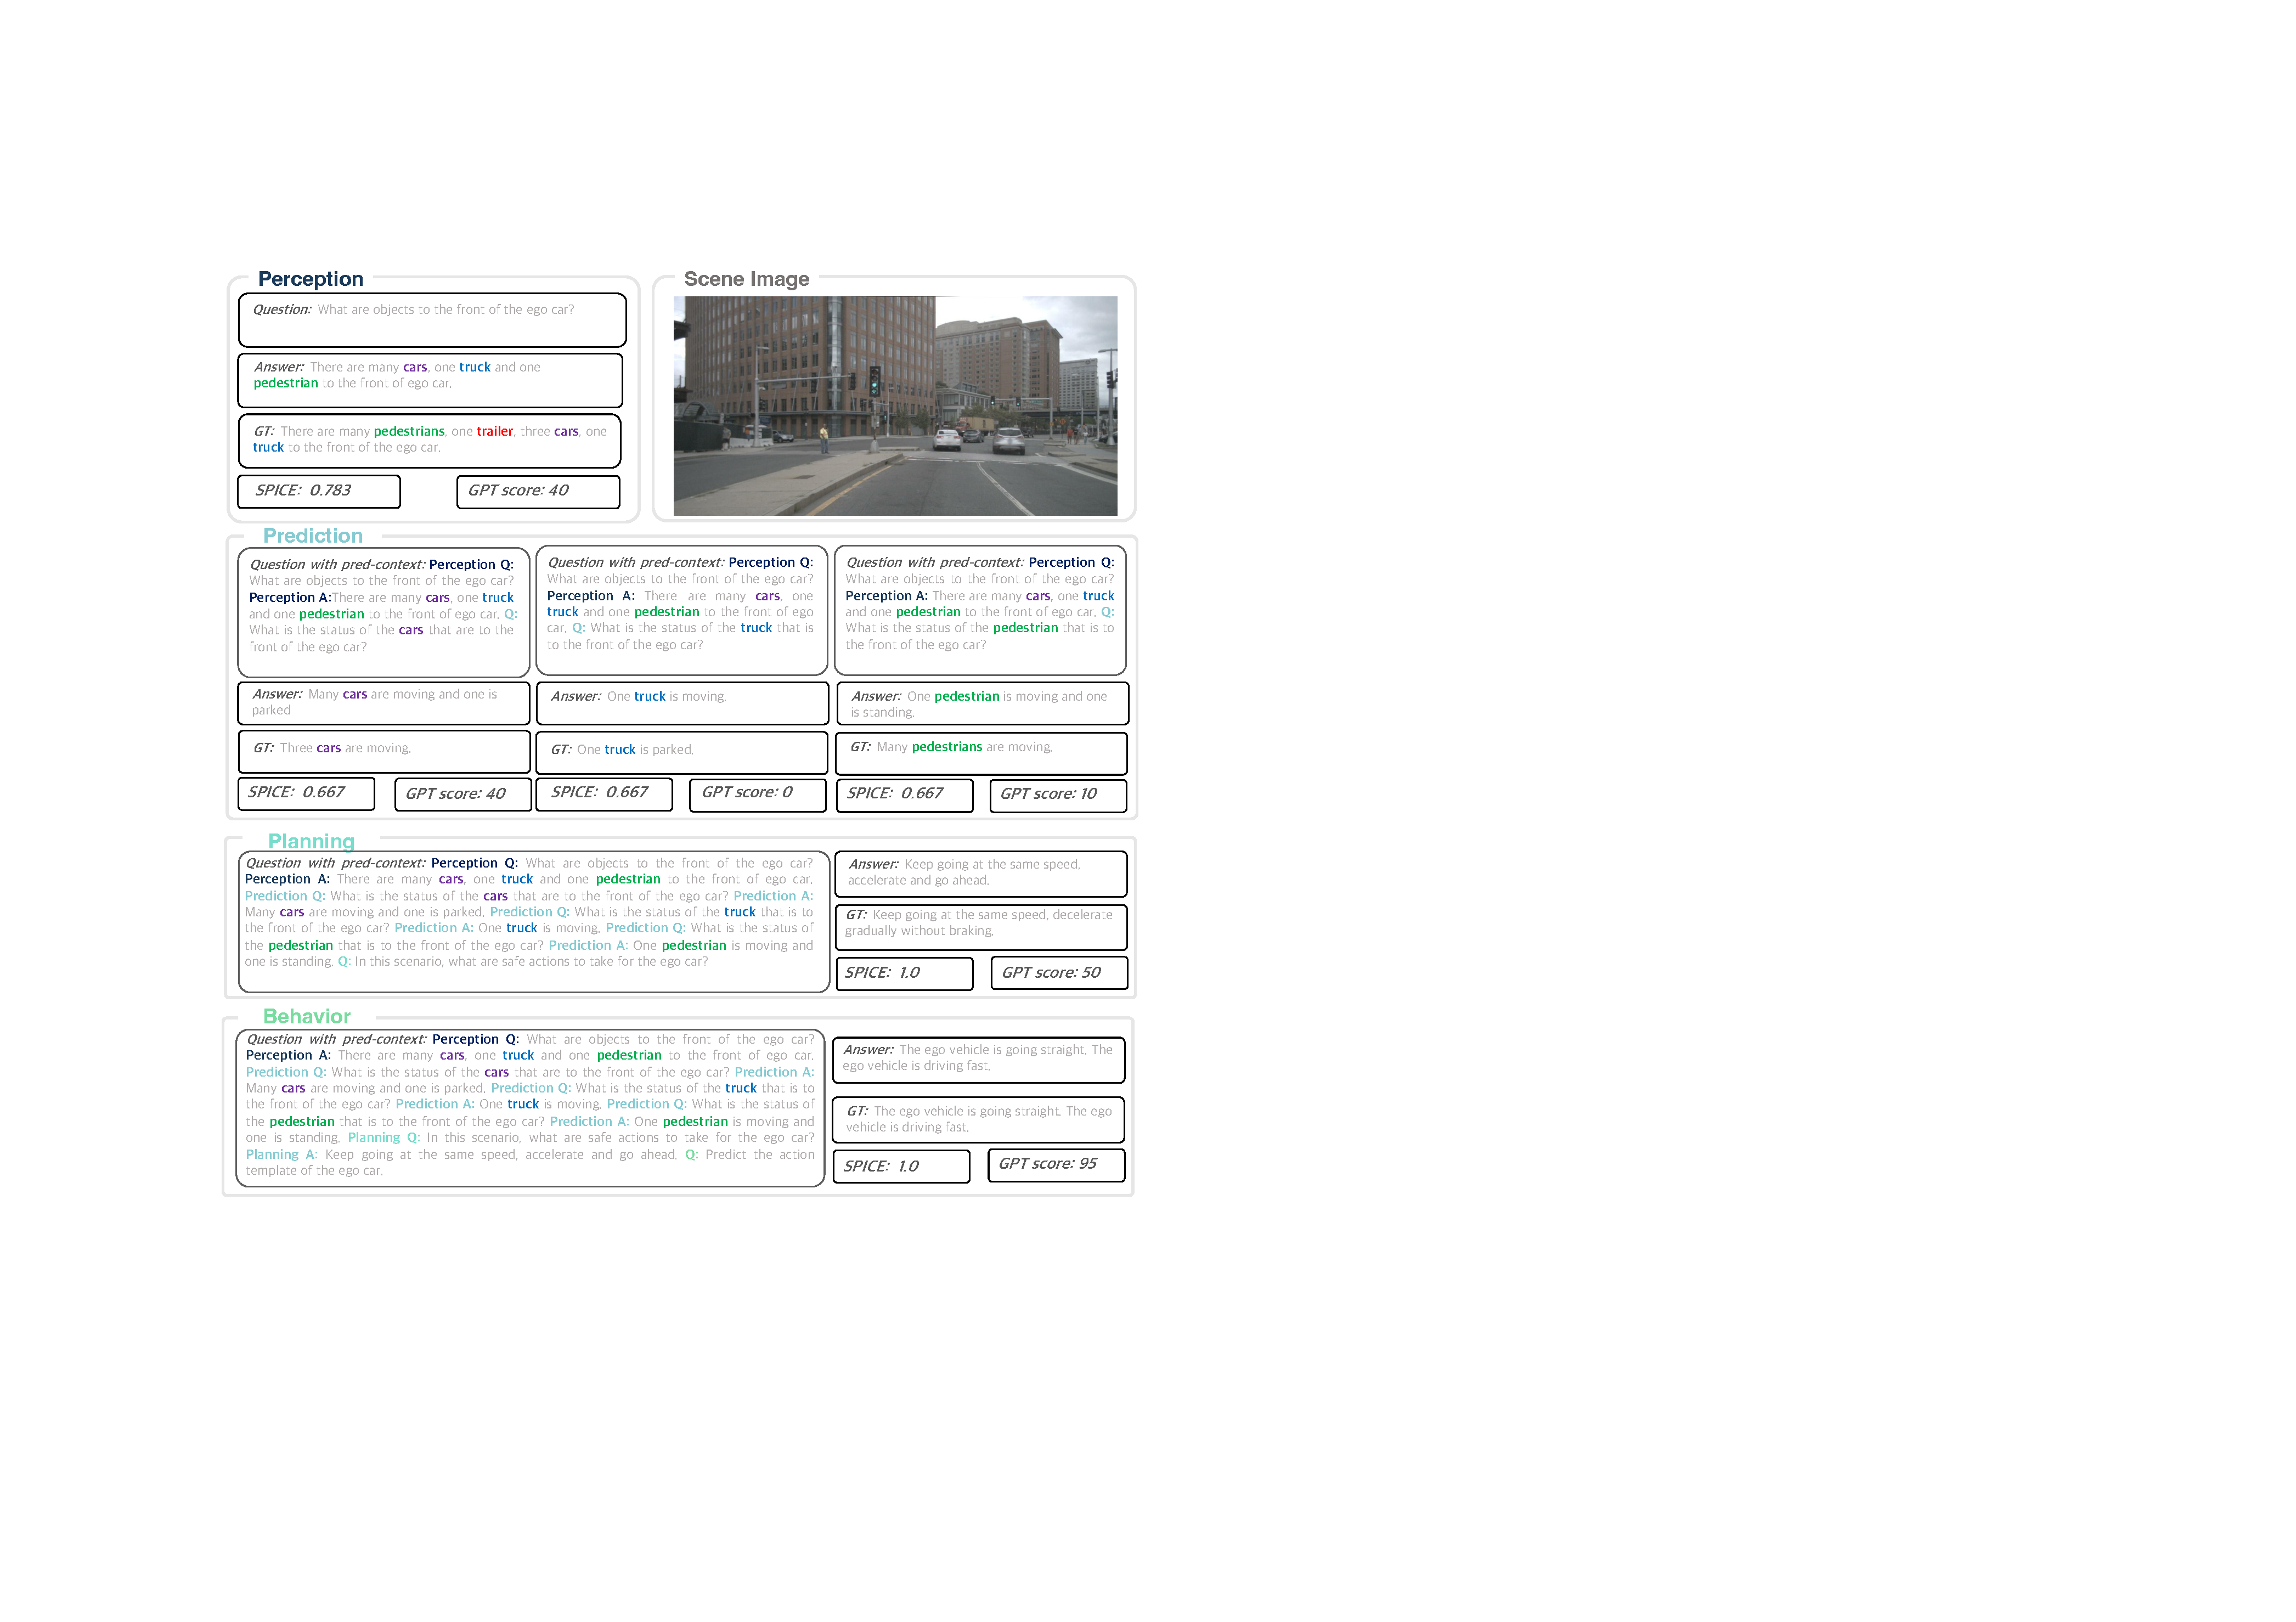
\includegraphics[width=\linewidth]{ch-drivelm/images/nus_detailed_results.pdf}
  \caption[Detailed qualitative results on DriveLM-nuScenes]{\textbf{Detailed qualitative results on DriveLM-nuScenes.} The graph prompting process can be divided into different tasks, and different QAs within each task revolve around different objects.}
  \label{drivelm:fig:nus_detailed_results}
\end{figure}

\begin{figure}[t]
  \centering
  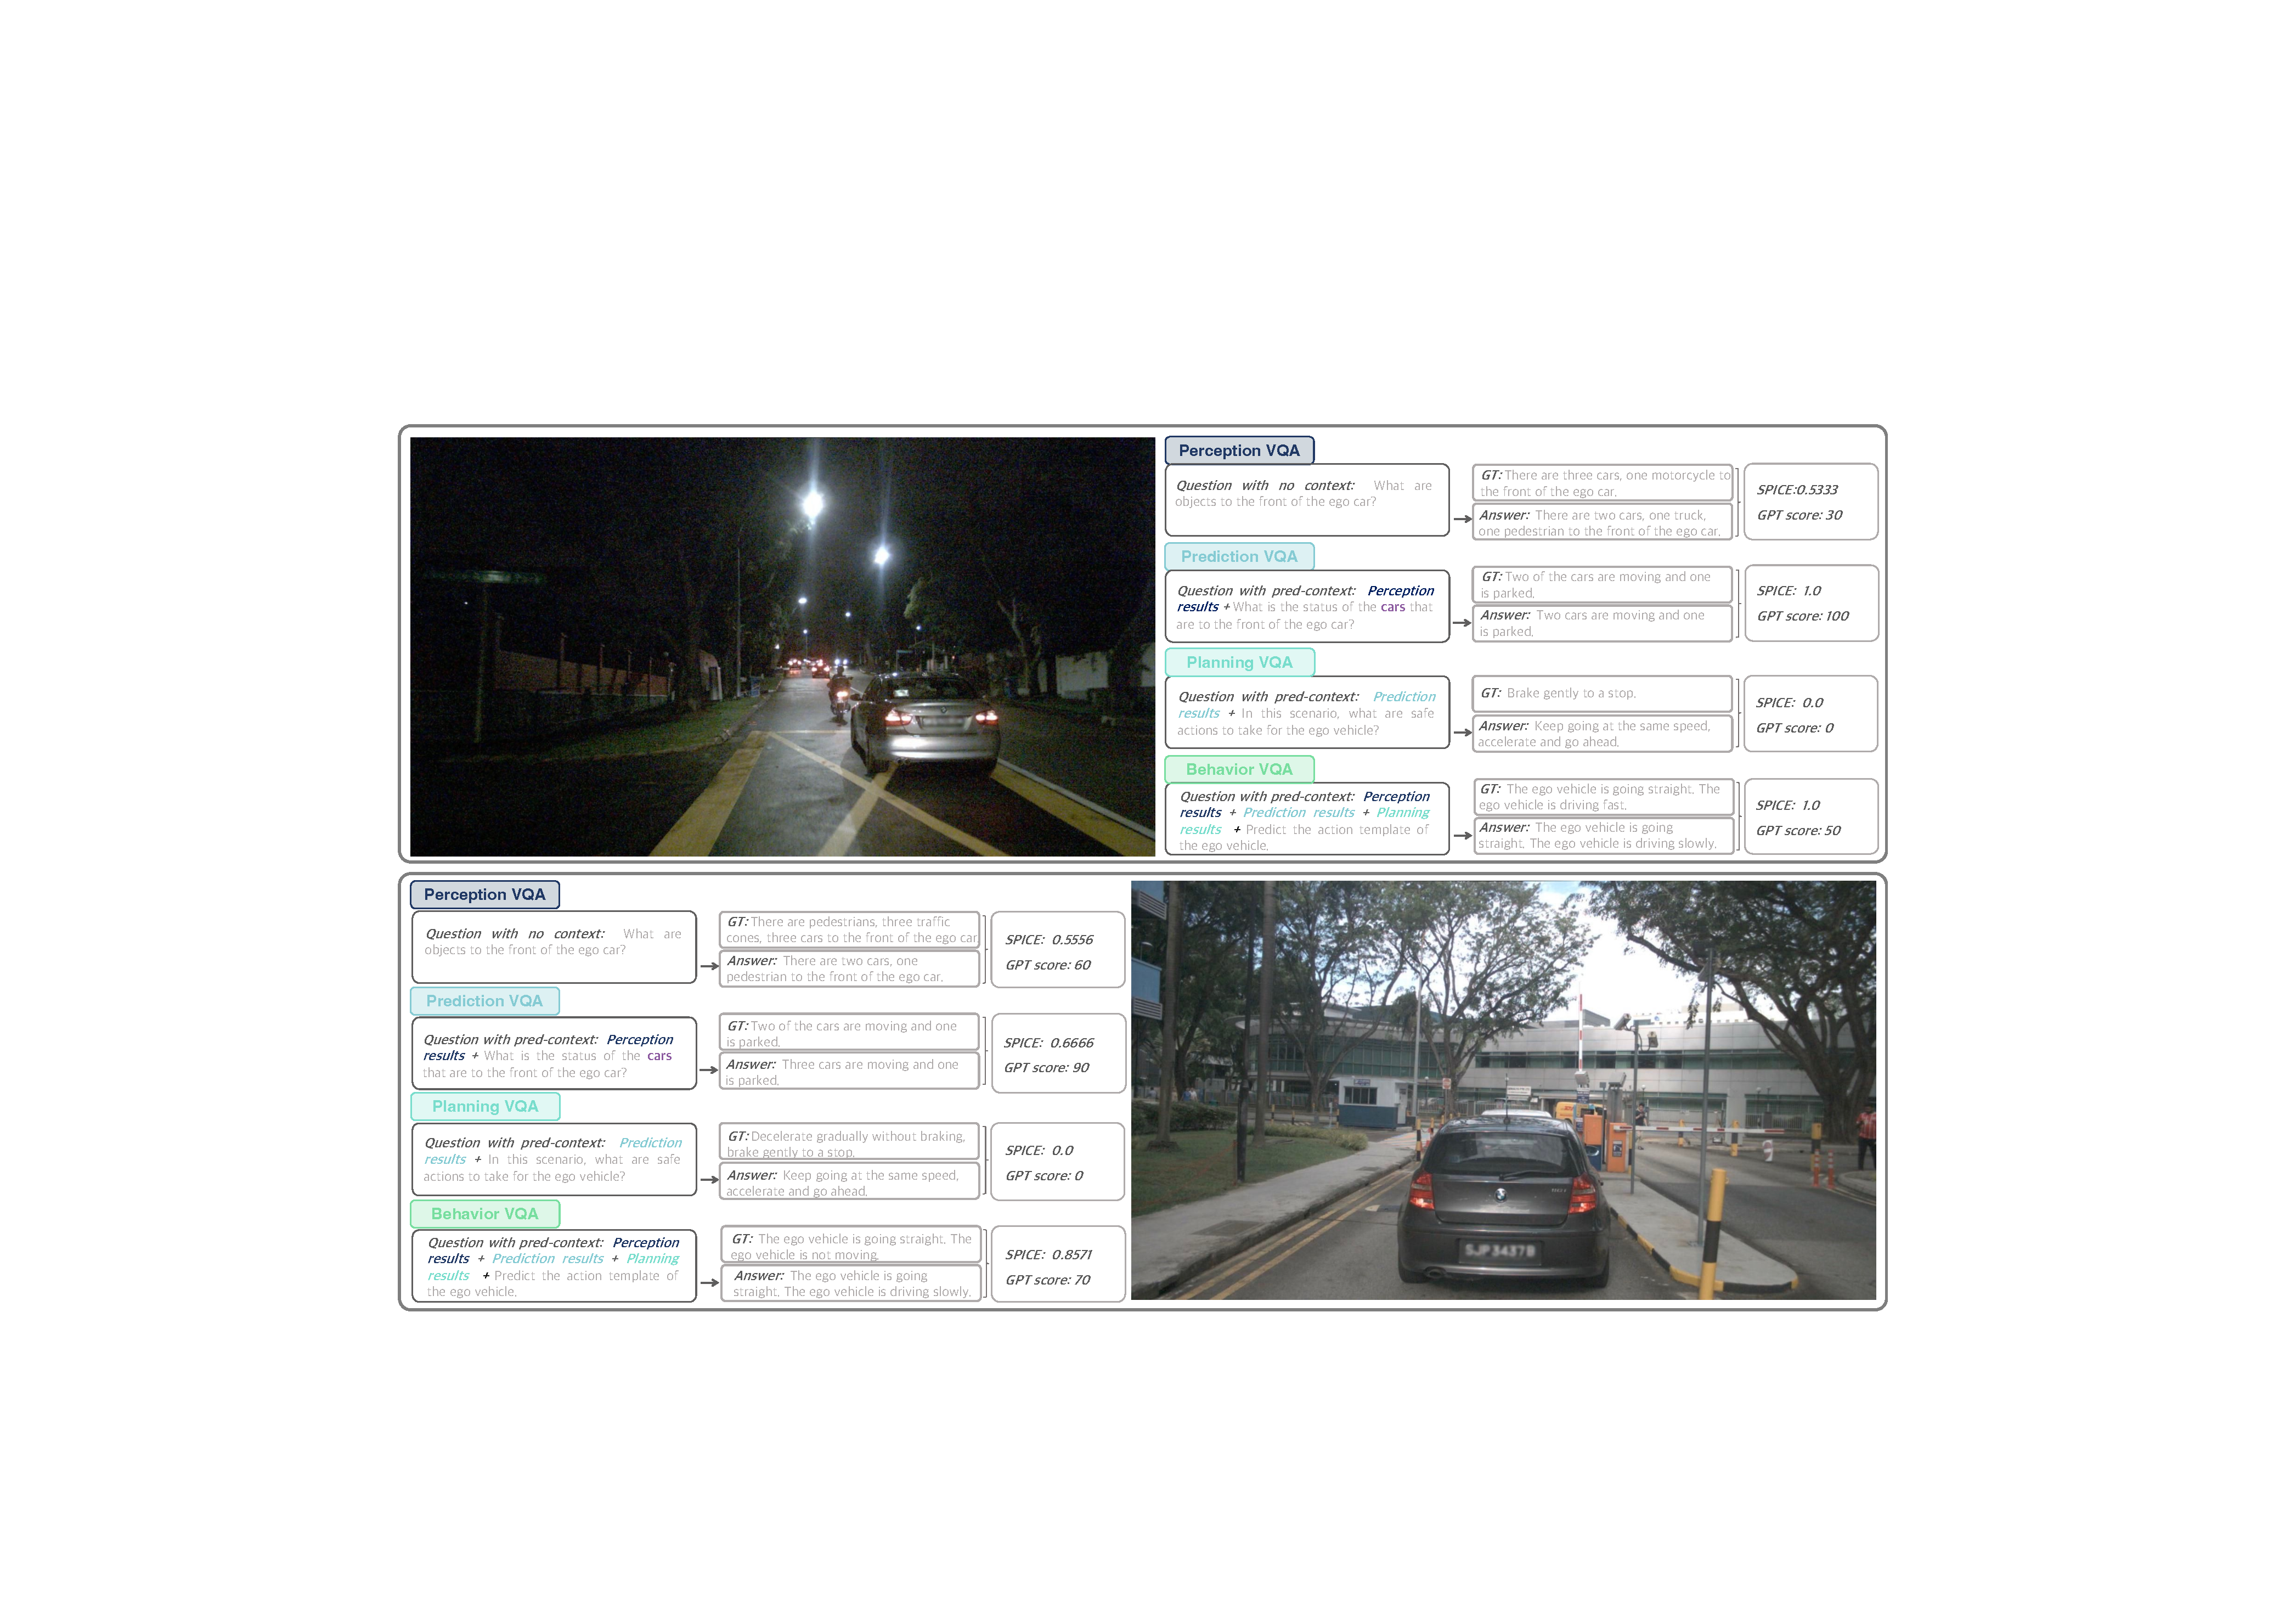
\includegraphics[width=\linewidth]{ch-drivelm/images/supp-vis-drivelm_1.pdf}
  \caption[More qualitative results on DriveLM-nuScenes]{\textbf{More qualitative results on DriveLM-nuScenes.} The examples illustrate the ability of DriveLM-Agent to perform VQA in driving scenarios.}
  \label{drivelm:fig:nus_results}
\end{figure}

\subsection{Waymo}\label{drivelm:app:qual_waymo}

Fig.~\ref{drivelm:fig:waymo_results} shows the results of the model trained on DriveLM-nuScenes when applied to Waymo, illustrating generalisation across sensor configurations. Since Waymo has no DriveLM annotations, the questions are defined as described in Appendix~\ref{drivelm:app:impl}, and no ground truth is available.

\begin{figure}[t]
  \centering
  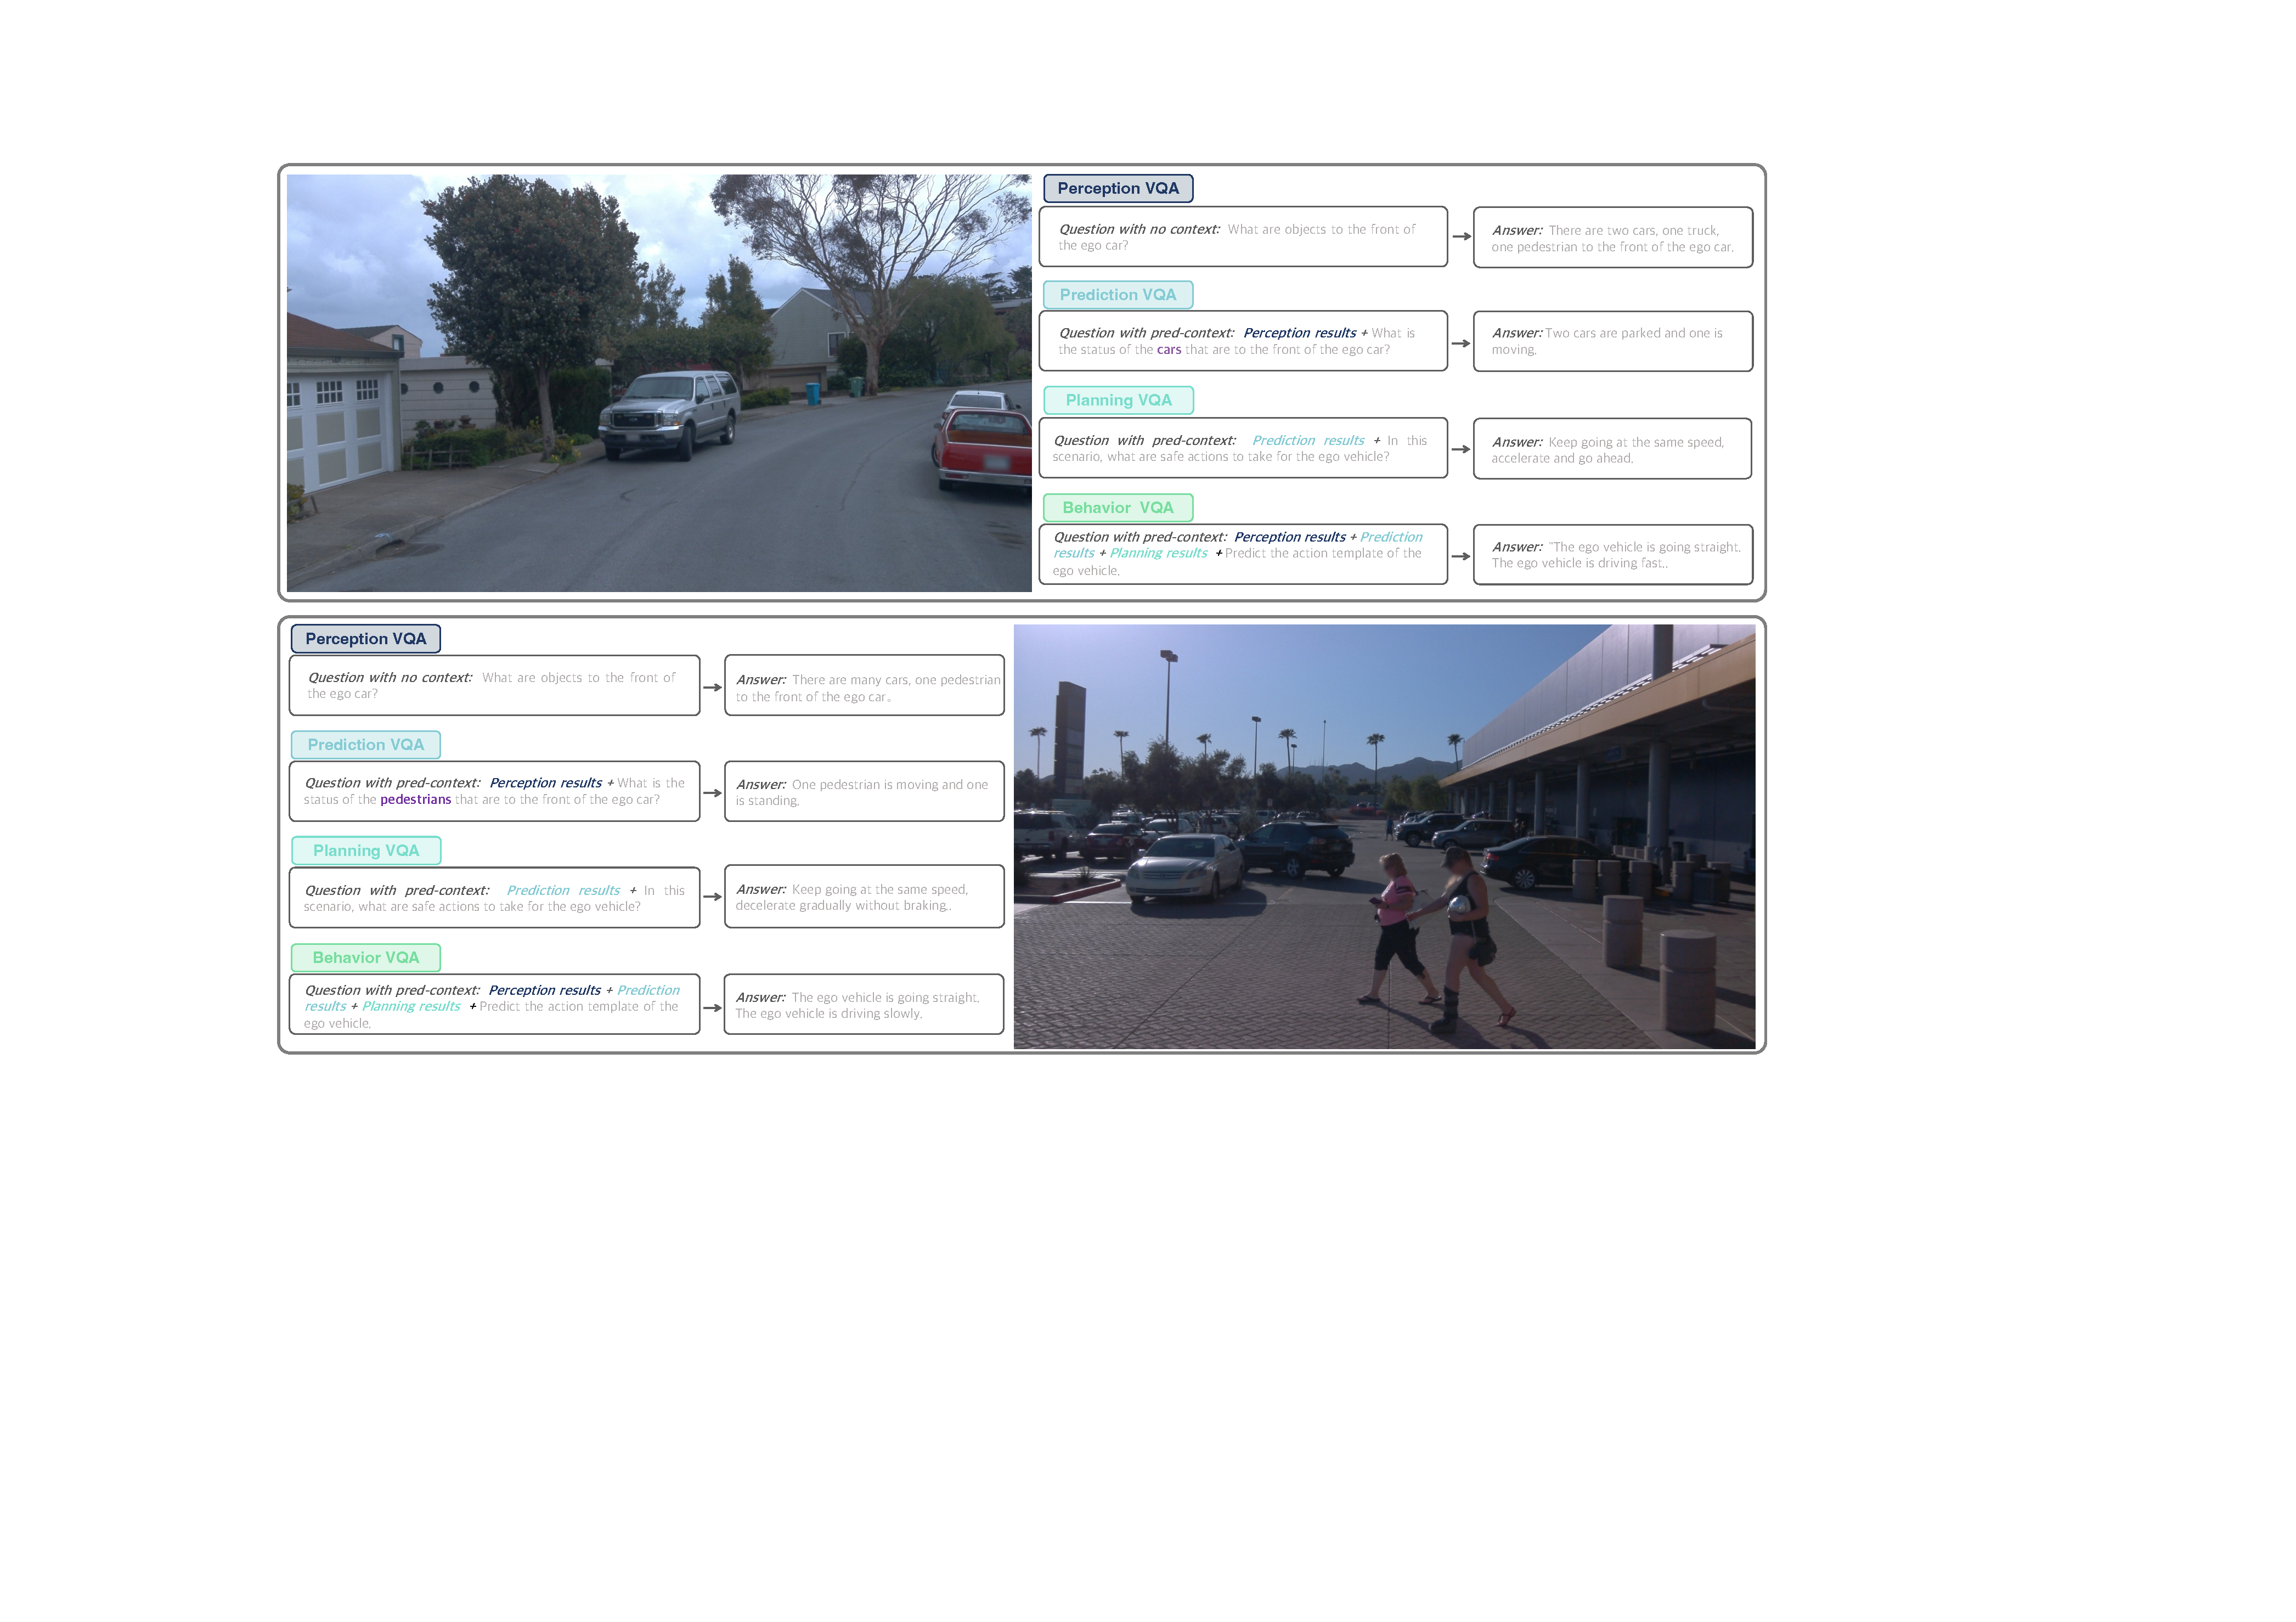
\includegraphics[width=\linewidth]{ch-drivelm/images/supp-vis-drivelm_2.pdf}
  \caption[Qualitative results on Waymo]{\textbf{Qualitative results on Waymo.} Two examples show how DriveLM-Agent generalises to a new sensor configuration.}
  \label{drivelm:fig:waymo_results}
\end{figure}

\subsection{DriveLM-CARLA}\label{drivelm:app:qual_carla}

\paragraph{Generalisation to the unseen pedestrian scenario.}
Fig.~\ref{drivelm:fig:carla_resultsPed} shows the generated behaviours on the generalisation test set with pedestrians. The first example, at the top, is a success: DriveLM-Agent recognises the pedestrian and infers the appropriate action, which in this case is to stop the vehicle. The behaviour stage interprets this context correctly, and the ego vehicle comes to a complete stop. The other two examples show the predominant failure modes of DriveLM-Agent in scenarios with pedestrians. In the middle example, the model still detects the pedestrian but fails to translate this detection into the correct behaviour. The bottom example shows a more severe limitation: the model completely overlooks the pedestrian and acts as if it did not exist, executing no evasive or stopping manoeuvre, which would pose a significant risk in the real world.

\paragraph{Graph visual question answering.}
Fig.~\ref{drivelm:fig:carla_resultsQA} shows two GVQA examples on DriveLM-CARLA; only a subset of the evaluated questions is shown. In the first example, the ego vehicle drives behind another vehicle, and the primary task is to follow the road and adapt the speed to the leading vehicle. DriveLM-Agent shows proficient scene understanding and identifies all important objects in the scene. Although the ground truth reveals that the CARLA simulator occasionally labels object colours incorrectly, DriveLM-Agent maintains reliable object recognition. The model also identifies the vehicle in front and reasons about what to do based on it. The second example takes place at an intersection regulated by a stop sign. DriveLM-Agent identifies all objects and reasons about the situation: it correctly determines that it must stop, not simply because of the stop sign but primarily because of a motorcycle positioned ahead. This suggests that DriveLM-Agent can prioritise dynamic obstacles over traffic control devices in some circumstances.

\begin{figure}[t]
  \centering
  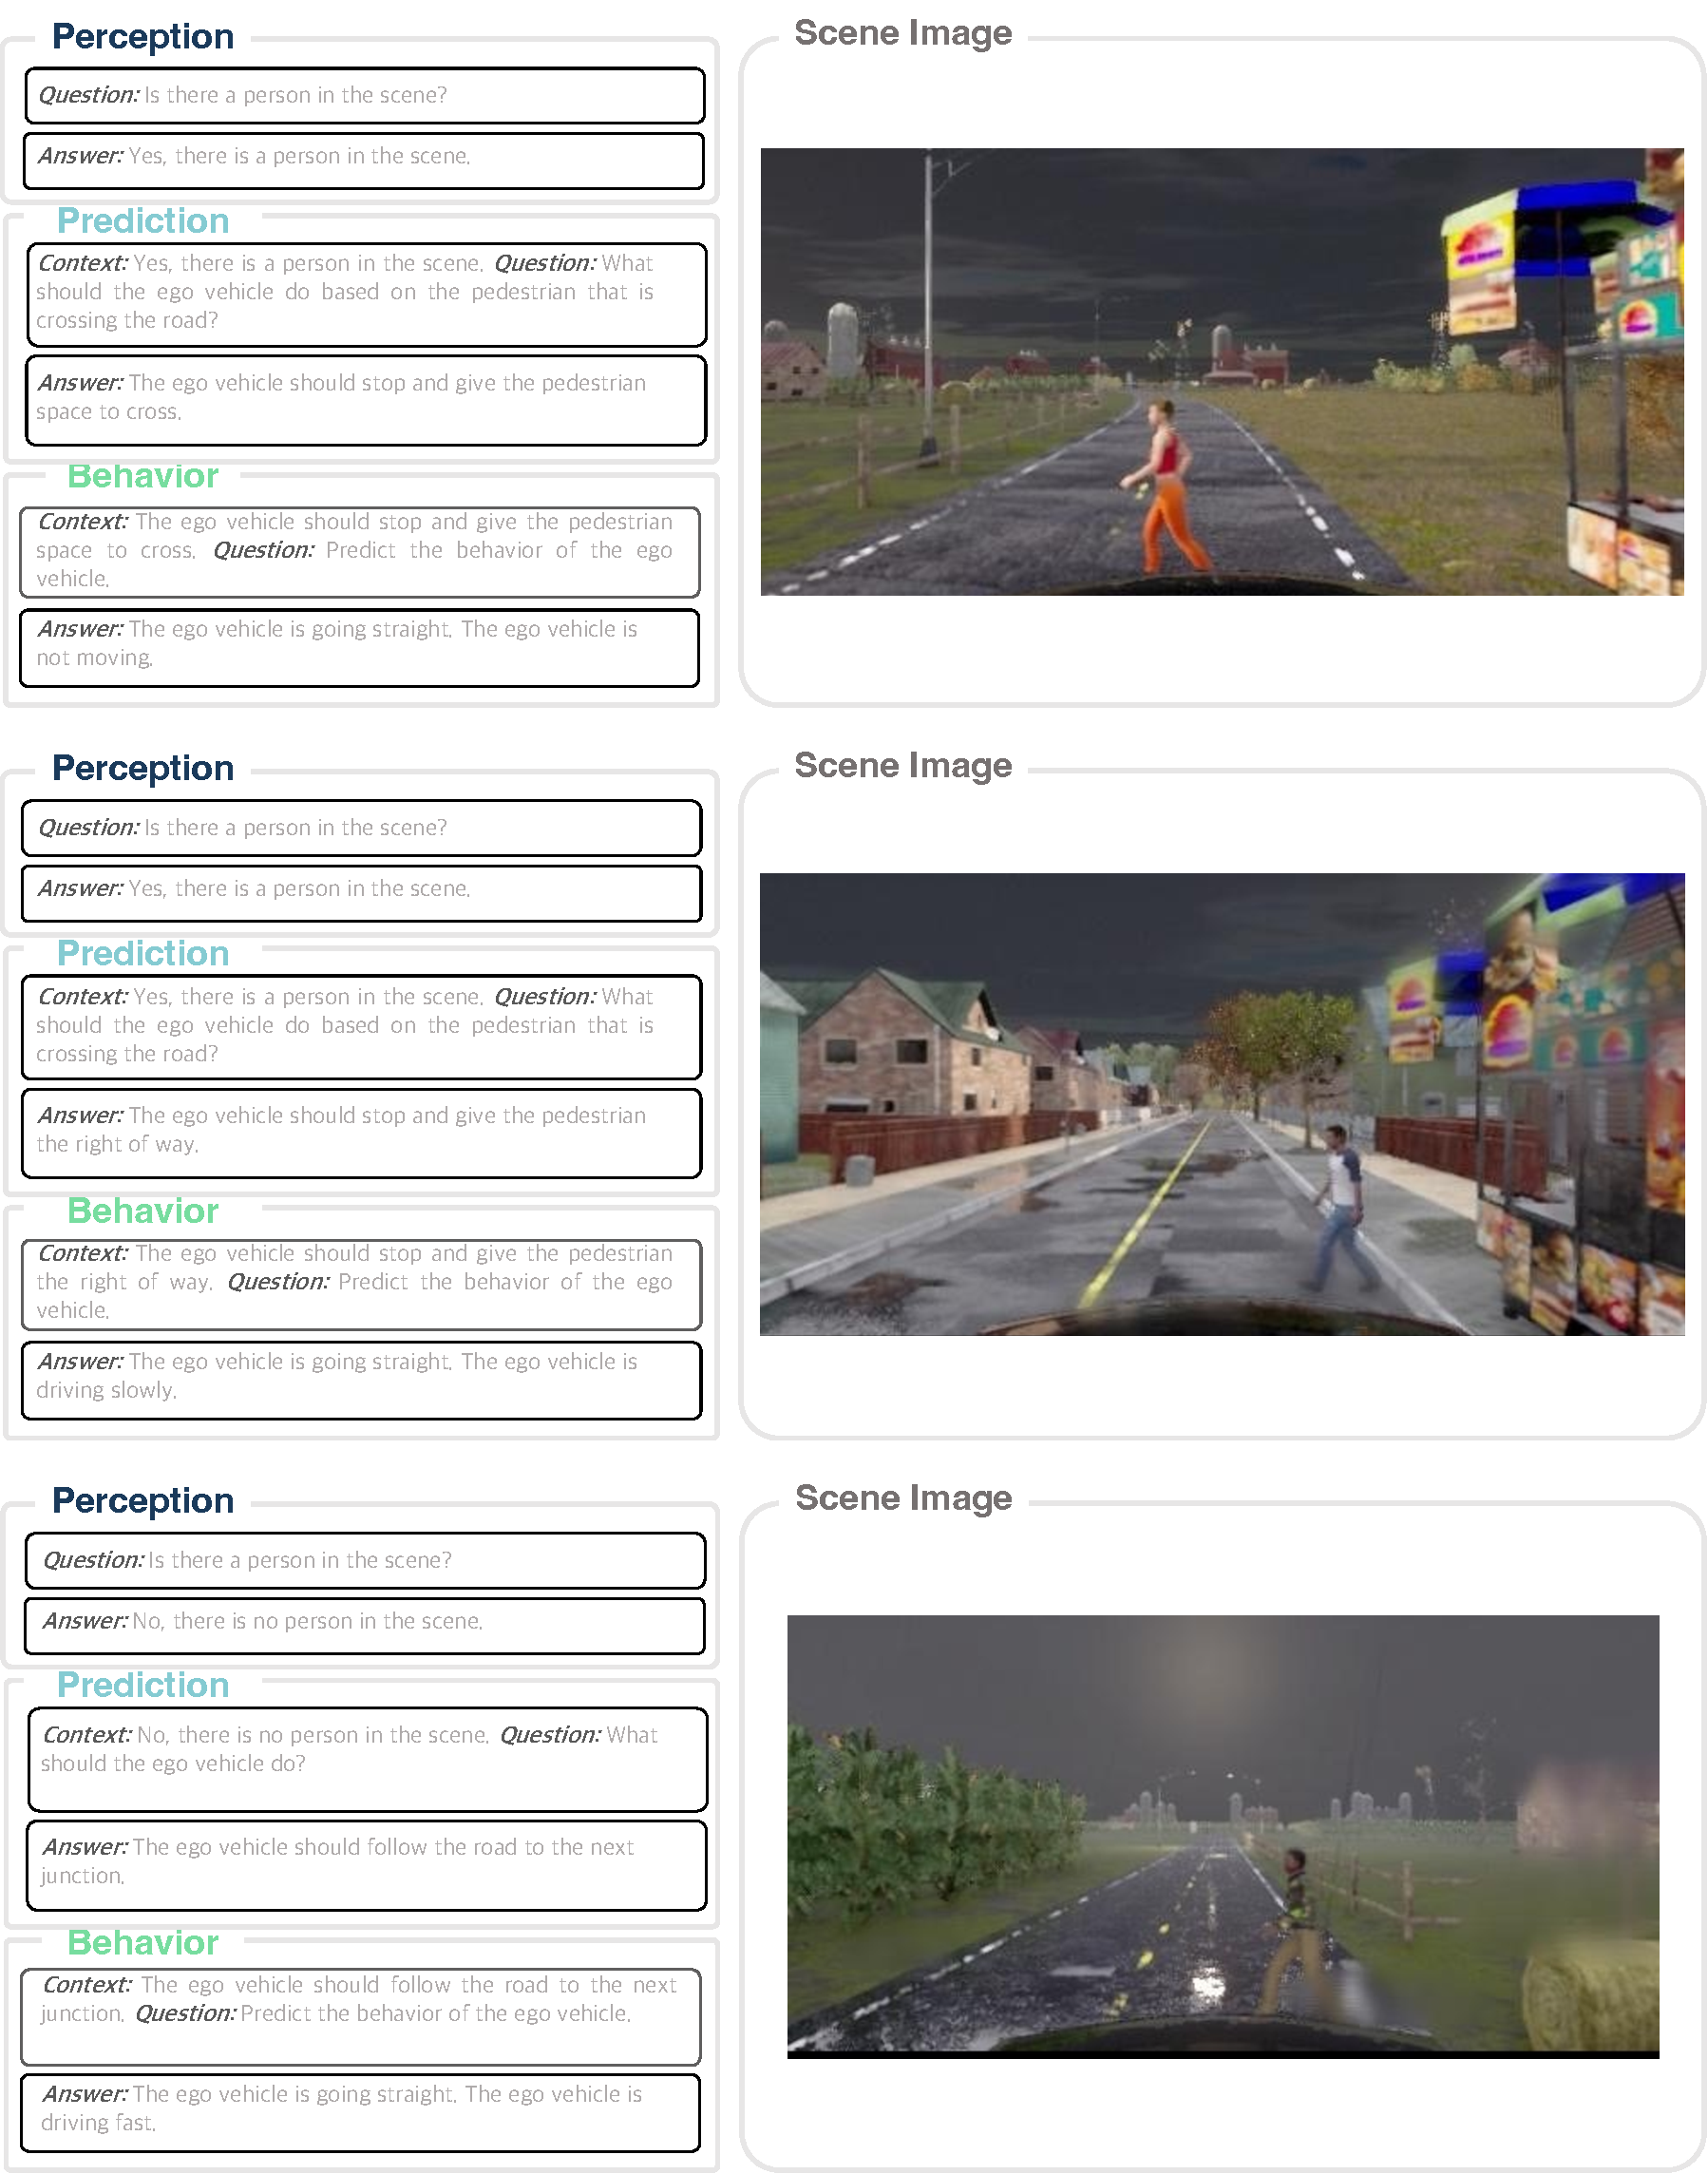
\includegraphics[width=0.9\linewidth]{ch-drivelm/images/carla_supp_2.pdf}
  \caption[Qualitative results on DriveLM-CARLA-ped]{\textbf{Qualitative results on the generalisation test set of DriveLM-CARLA.} Three examples of DriveLM-Agent in the pedestrian scenario. The first example shows a success case, and the second and third show two common failure cases of the model.}
  \label{drivelm:fig:carla_resultsPed}
\end{figure}

\begin{figure}[t]
  \centering
  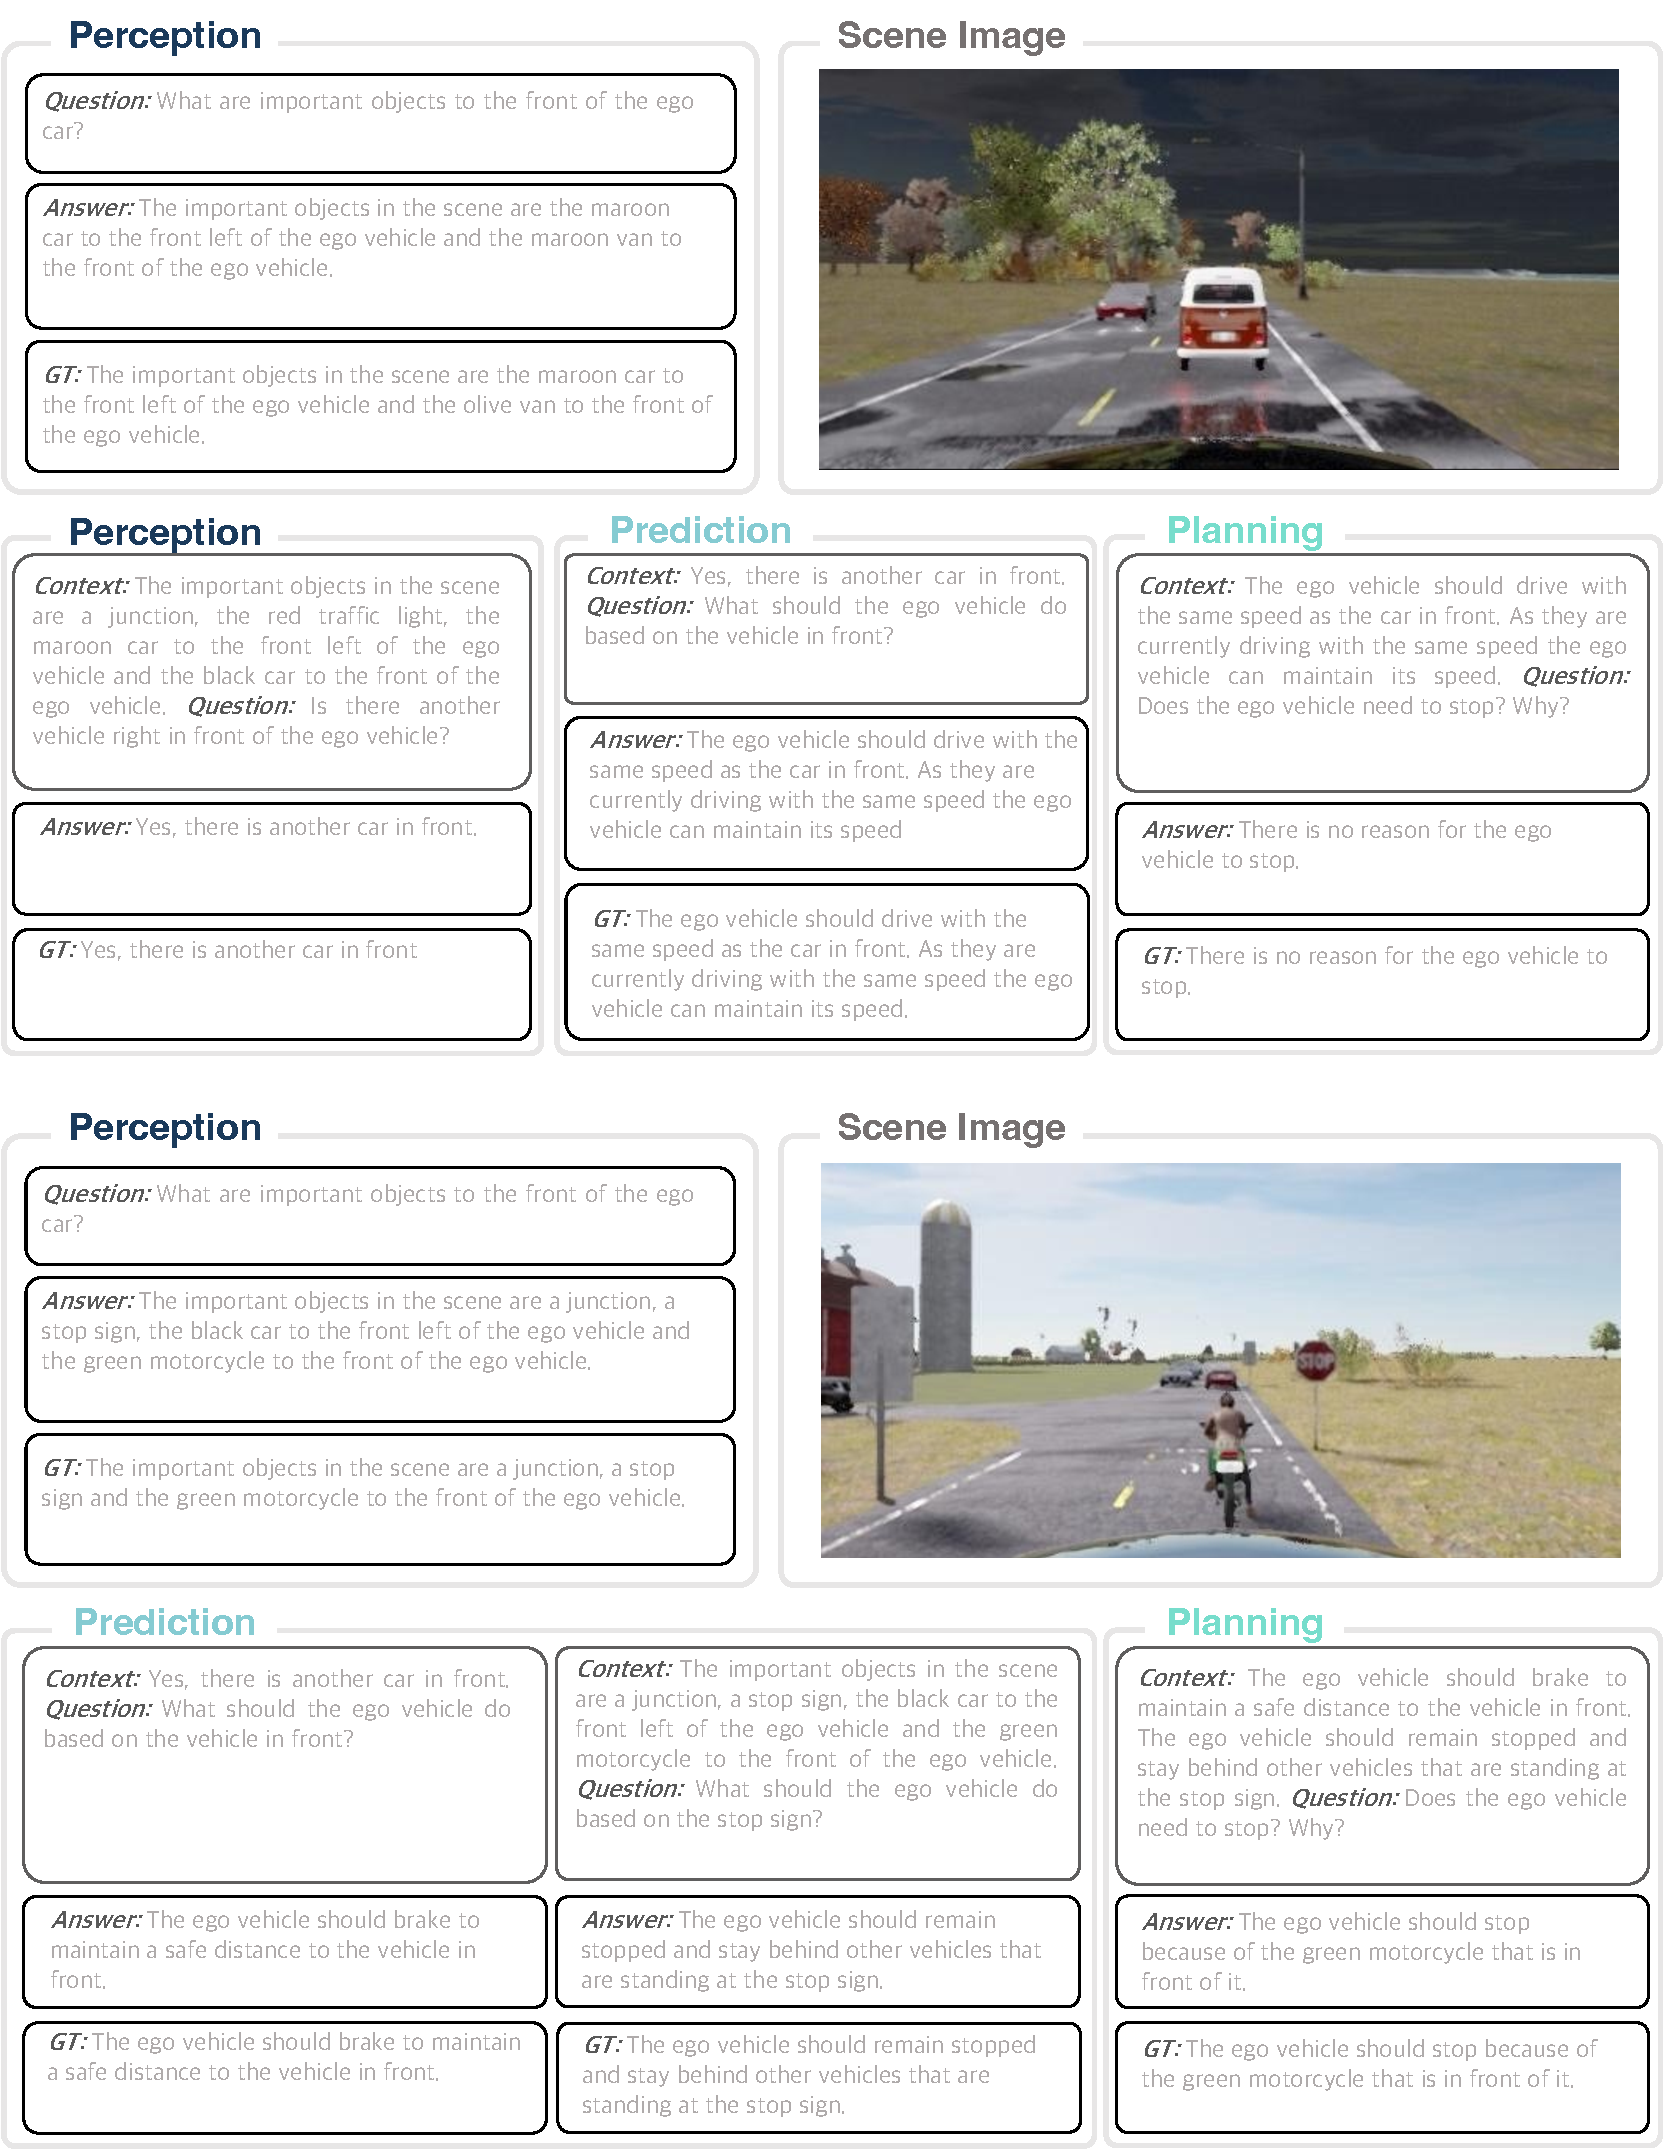
\includegraphics[width=0.9\linewidth]{ch-drivelm/images/carla_supp_1.pdf}
  \caption[Qualitative VQA results on DriveLM-CARLA]{\textbf{Qualitative VQA results on DriveLM-CARLA.} The first example shows how DriveLM-Agent deals with a vehicle directly in front of the ego vehicle. The second example shows an intersection with a stop sign and other traffic participants waiting in front of the ego vehicle at the stop sign.}
  \label{drivelm:fig:carla_resultsQA}
\end{figure}

\section{Broader Impact}\label{drivelm:app:impact}

We believe that this approach can accelerate progress in autonomous driving by allowing it to benefit directly from better VLMs. Our goal is to make progress towards autonomous driving, which will have a profound impact if successful. By bringing VLMs into this area, we accept their ethical implications, such as hallucinations and high resource use. Yet, by improving the interactivity between humans and autonomous driving systems, we can build confidence in the technology. This could hasten its acceptance and lead to safer transportation in the long term.
